\documentclass[russian,utf8,nocolumnsxix,nocolumnxxxi,nocolumnxxxii]{eskdtext}
\makeatletter
\newcommand{\updateStamp}{%
\savebox{\ESKD@stamp@ii@box}{%
\setlength{\unitlength}{1mm}%
\begin{picture}(0,0)(0,0)
\linethickness{\ESKDlineThick}
\put(0,40){\line(1,0){185}}
\put(0,30){\line(1,0){65}}
\put(0,25){\line(1,0){185}}
\put(135,20){\line(1,0){50}}
\put(135,15){\line(1,0){50}}
\linethickness{\ESKDlineThin}
\put(0,35){\line(1,0){65}}
\multiput(0,20)(0,-5){4}{\line(1,0){65}}
\linethickness{\ESKDlineThick}
\put(0,0){\line(0,1){40}}
\put(7,25){\line(0,1){15}}
\put(17,0){\line(0,1){40}}
\put(40,0){\line(0,1){40}}
\put(55,0){\line(0,1){40}}
\put(65,0){\line(0,1){40}}
\put(135,0){\line(0,1){25}}
\put(140,15){\line(0,1){5}}
\put(145,15){\line(0,1){5}}
\put(150,15){\line(0,1){10}}
\put(165,15){\line(0,1){10}}
\put(67, 1){\parbox[b][23mm][c]{66mm}{\centering\ESKDfontIII\ESKDtheColumnI}}
\put(67, 26){\parbox[b][13mm][c]{106mm}{\centering\ESKDfontVII\ESKDtheColumnII}}
\put(135, 21.3){\makebox[15mm]{\ESKDfontIII\ESKDcolumnIVname}}
\put(135, 16.3){\makebox[5mm][c]{\ESKDfontIII\ESKDtheColumnIVfI}}
\put(140, 16.3){\makebox[5mm][c]{\ESKDfontIII\ESKDtheColumnIVfII}}
\put(145, 16.3){\makebox[5mm][c]{\ESKDfontIII\ESKDtheColumnIVfIII}}
\put(150, 21.3){\makebox[15mm]{\ESKDfontIII%
  \ifESKD@twoside\ESKDcolumnVIItwosideName\else\ESKDcolumnVIIname\fi}}
\put(165, 21.3){\makebox[20mm]{\ESKDfontIII%
  \ifESKD@twoside\ESKDcolumnVIIItwosideName\else\ESKDcolumnVIIIname\fi}}
\put(137, 1){\parbox[b][13mm][c]{46mm}{\centering\ESKDfontV\ESKDtheColumnIX}}
\put(0.5, 21.3){\makebox[16mm][l]{\ESKDfontIII\ESKDcolumnXfIname}}
\put(0.5, 16.3){\makebox[16mm][l]{\ESKDfontIII\ESKDcolumnXfIIname}}
\put(0.5, 11.3){\makebox[16mm][l]{\ESKDfontIII\ESKDcolumnXfIVname}}
\put(0.5, 6.3){\makebox[16mm][l]{\ESKDfontIII\ESKDcolumnXfVname}}
\put(0.5, 1.3){\makebox[16mm][l]{\ESKDfontIII\ESKDcolumnXfVIname}}
\put(17.5, 21.3){\makebox[22mm][l]{\ESKDfontIII\ESKDtheColumnXIfI}}
\put(17.5, 16.3){\makebox[22mm][l]{\ESKDfontIII\ESKDtheColumnXIfII}}
\put(17.5, 11.3){\makebox[22mm][l]{\ESKDfontIII\ESKDtheColumnXIfIV}}
\put(17.5, 6.3){\makebox[22mm][l]{\ESKDfontIII\ESKDtheColumnXIfV}}
\put(17.5, 1.3){\makebox[22mm][l]{\ESKDfontIII\ESKDtheColumnXIfVI}}
\put(0, 26.3){\makebox[7mm]{\ESKDfontIII\ESKDcolumnXIVname}}
\put(7, 26.3){\makebox[10mm]{\ESKDfontIII\ESKDcolumnXVname}}
\put(17, 26.3){\makebox[23mm]{\ESKDfontIII\ESKDcolumnXVIname}}
\put(40, 26.3){\makebox[15mm]{\ESKDfontIII\ESKDcolumnXVIIname}}
\put(55, 26.3){\makebox[10mm]{\ESKDfontIII\ESKDcolumnXVIIIname}}
\end{picture}}}
\makeatother

% В рамке в поле с title уменьшить шрифт.
\renewcommand{\ESKDtheColumnI}{\ESKDfontIII\ESKDtheTitle\par\ESKDtheDocName}

\ESKDdepartment{Министерство образования РФ}
\ESKDcompany{Пензенский Государственный Университет}
\ESKDclassCode{31 1398}
\ESKDtitle{Распределенная агентно-ориентированная система доступа к базам данных}
\ESKDdocName{Технические условия}
\ESKDsignature{АБВГД ХХХХХХХХ}
\ESKDauthor{Теренков~А.С.}
\ESKDtitleApprovedBy{%
a}{Гусев~И.~И.}
\ESKDtitleAgreedBy{%
a}{Иванов~И.~И.}
\ESKDtitleDesignedBy{%
a}{Теренков~А.С.}
\ESKDtitleDesignedBy{%
a}{Зинкин~С.А.}
\ESKDchecker{Зинкин~С.А.}
\ESKDnormContr{Кучин~А.В.}
\usepackage{tocloft}
\usepackage{graphicx}
\usepackage{listings}
\usepackage{eskdtotal}
\lstset{breaklines=true}
\lstset{basicstyle=\small\ttfamily}
\lstset{lineskip={-1.5pt}}
\captionsetup{font=small}
\graphicspath{{chapter0/}{chapter1/}{chapter2/}{chapter3/}}
\sloppy
\begin{document}
\ESKDdocName{Реферат}
\updateStamp
\ESKDthisStyle{formII}
\section*{Реферат}
\addcontentsline{toc}{section}{Реферат}
Пояснительная записка содержит \_\_ листов формата А4, \_ рисунков, \_ таблиц, 6 листов формата А1, 2 плаката формата А1, 10 источников, 4 приложения.

Распределенная агентно-ориентированная система доступа к базам данных.

РАСПРЕДЕЛЕННЫЕ ВЫЧИСЛИТЕЛЬНЫЕ СИСТЕМЫ, ПРОГРАММНЫЕ АГЕНТЫ, JADE, JAVA, БАЗЫ ДАННЫХ

Объектами исследования являются: распределенные системы, программные агенты, автоматизированный подход к сборке и развертыванию проектов.

Цель работы~--- разработка распределенной системы доступа к базам данных на основе технологии программных агентов.

В результате проведенной работы был реализован проект, удовлетворяющий поставленной задаче.

В пояснительной записке выполнено описание базовых понятий теории распределенных вычислительных систем, сделан обзор современных подходов к построению подобных решений,  представлено изложение принципов  автоматизированной сборки и развертывания приложений и рассмотрена работа с фреймворком Maven.

Графическая часть содержит модели UML.

\newpage
\section*{Список терминов и сокращений}
АОП~--- агентно-ориентированное программирование.

МАС~--- мультиагентная система.
 
ВС~--- вычислительная система.

СУБД~--- система управления базами данных.

ПЭВМ~--- персональная электронно-вычислительная машина.

UML (Unified Modeling Language)~--- унифицированный язык моделирования.

\maketitle
\newpage
\renewcommand{\cftsecleader}{\cftdotfill{\cftdotsep}}
\tableofcontents
\newpage
\ESKDdocName{Введение}
\updateStamp
\ESKDthisStyle{formII}
\section*{Введение}
\addcontentsline{toc}{section}{Введение}
Процессы мировой глобализации неразрывно связаны с развитием вычислительной техники и информационных технологий. Классические задачи, решаемые в рамках обособленного вычислительного узла, вытесняются задачами, требующими взаимной коммуникации и обмена ресурсами между инфомационными системами. В свою очередь это ведет к постоянному увеличению требований к имеющимся подходам и технологиям, предоставляющим подобные решения.

Одним из ведущих направлений в этой области является создание распределенных вычислительных систем, способных решать сложные и масштабные задачи путем взаимного сотрудничества и взаимодействия. Однако не любая совокупность объединеных компьютеров способна предоставить эффективный механизм решения крупных научных, производственных и технологических задач, поскольку, как показывают исследования, от подобных систем в процессе и принципах их функционирования требуется обеспечение следующего набора основных требований:

\begin{enumerate}
\item не требовать использования дополнительного дорогостоящего коммутационного оборудования;
\item быть достаточно простой в настройке и эксплуатации; не требовать для постоянного обслуживания высококлассных специалистов;
\item быть <<прозрачной>> для конечного пользователя, т.е. должна скрывать от него все тонкости ее функционирования;
\item быть <<самонастраиваемой>>, т.е. уметь поддерживать себя в активном состоянии в любых ситуациях (за исключением форсмажорных) без вмешательства человека;
\item поддерживать выполнение задач широкого класса;
\item быть надежно защищенной от вторжения извне.
\end{enumerate}

Вышеприведенный набор требований как нельзя лучше реализуется в рамках современной и перспективной концепции программных агентов, разработанных для решения сложных и масштабных проблем и задач. Одной из попыток показать это на реальном примере и является создение распределенной системы доступа к базам данных на основе агентно-ориентированного подхода в рамках данного курсового проекта. Перед этим будут описаны общие положения и теоретические основы данной предметной области, выполнено краткое описание современных подходов для решения подобных задач, их архитектурных особенностей, ключевых преимуществ и недостатков.

Также будет подробно описан агентно-ориентированный подход к программированию, показаны механизмы функционирования агентов, изучены их основные свойства и методы. Кроме того, будут рассмотрены принципы взаимодействия агентов между собой и их жизненные циклы.

Заключительным этапом проекта станет процесс непосредственной реализации работоспособной системы на основе программной среды разработки мультиагентных систем и приложений JADE, способной автономно функционировать в рамках поставленной задачи, предоставляя конечному пользователю унифицируемый доступ к имеющейся инфомации, расположенной на множестве компьютеров в сети.

Стоит отметить высокую актуальность рассматриваемой тематики, ее востребованность на современном рынке инфомационных технологий и программного обеспечения, а также недостаточную изученность и распространенность в широких кругах как в нашей стране, так за рубежом. Данный дипломный проект может послужить еще одним, пусть и небольшим вкладом среди пока еще узкого круга работ и материалов в области изучения, развития и реализации подхода построения распределенных вычислительных систем с использованием технологии программных агентов.

\section{Обзор предметной области и выбор инструментальной платформы}
\subsection{Распределенные вычислительные системы}
Парадигма распределенных вычислительных систем в настоящее время характеризуется стремительными темпами развития и эволюции используемых в ней идеологий и подходов. За непродолжительное время существования систем такого типа появилось множество различных схем организаций распределенных вычислений, набравших большой вес и общее признание, но практически исчезнувших впоследствии под давлением более новых и модных подходов. Такая ситуация зачастую ведет к тому, что исчезнувшая из виду технология появляется вновь под новым именем. В результате происходит непрерывное перемешивание базовых концепций с новейшими наработками. Для изучения и систематизации имеющихся технологий и подходов необходимо разобраться с базовыми понятиями и принципами организации систем подобного направления. 

\subsubsection{Понятие распределенной системы}
По утверждению известного специалиста в области информатики Э. Таненбаума, не существует общепринятого и в то же время строгого определения распределенной системы. 

Зачастую, при определении понятия <<распределенная система>> главное место отводят принципу разделения функционала между несколькими компьютерами. Однако при таком подходе распределенной является любая вычислительная система, в которой обработка данных разделена между двумя и более компьютерами. Сам Э.~Таненбаум в узком смысле определяет распределенную систему как набор соединенных каналами связи независимых компьютеров, которые с точки зрения пользователя некоторого программного обеспечения выглядят как единое целое.

\begin{figure}[h]
\center{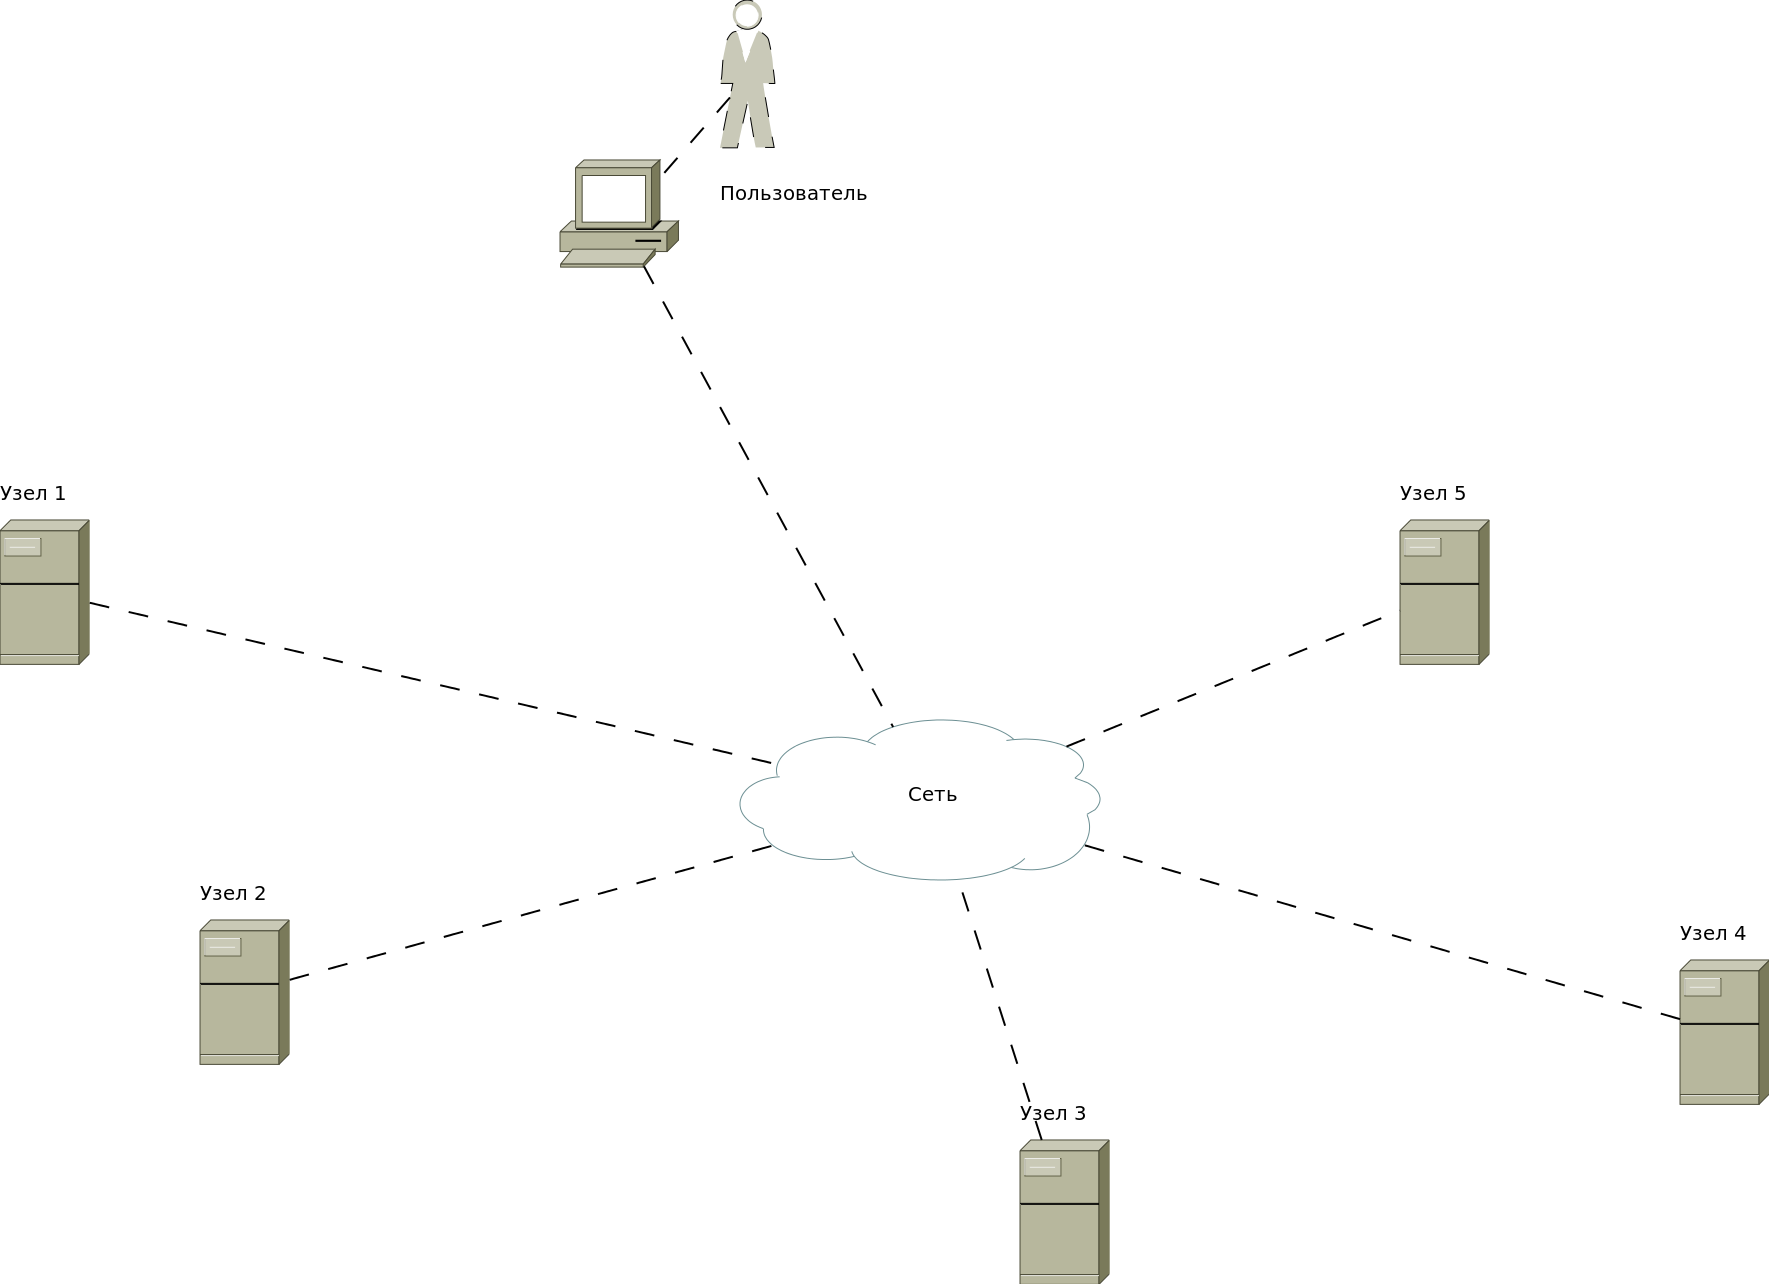
\includegraphics[width=1\linewidth]{dcs}}
\caption{Архитектура распределенной системы}
\label{0:dcs}
\end{figure}

В распределенных системах ключевым моментом является скрытие от пользователей различий между компьютерами и принципов организации их соединений (пользователь может даже не знать, что компьютер, используемый в системе, всего один). Пользователи и приложения единообразно работают в распределенных системах, независимо от того, где и когда происходит их взаимодействие. Вычислительная система, состоящая из множества различных вычислительных машин, на которых установлено различное программное обеспечение, может называться распределенной системой только в том случае, если для своих пользователей она выглядит и ведет себя как классическая однопроцессорная система с разделением времени. Чтобы поддерживать представление различных компьютеров и вычислительных сетей в виде единой системы, организация распределенных систем часто включает в себя дополнительный уровень программного обеспечения. Этот уровень называется уровнем системной поддержки.

Основная задача распределенных систем программного обеспечения~--- облегчить их пользователям доступ к удаленным ресурсам, а также организовывать их одновременное бесконфликтное использование. Зачастую, в классических системах совместное использование ресурсов достигается за счет тесного взаимодействия пользователей системы. Однако пользователь распределенной системы не должен знать, что он является не единственным ее пользователем. Ресурсы при этом могут быть как виртуальными, так и <<традиционными>>~--- компьютеры, принтеры, устройства хранения файлов и т.д.

\subsubsection{Основные понятия распределенных вычислительных систем}
\begin{enumerate}
\item Ресурс. Ресурсом называется любая программная или аппаратная сущность, представленная или используемая в распределенной сети. Например, компьютер, устройство хранения, файл, коммуникационный канал, сервис и т.п.
\item Узел~--- любое аппаратное устройство в распределенной вычислительной системе.
\item Сервер~--- это поставщик информации в распределенной вычислительной системе (например, веб-сервер).
\item Клиент~--- это потребитель информации в распределенной вычислительной системе (например, веб-браузер).
\item Пир~--- это узел, совмещающий в себе как клиентскую, так и серверную часть (т.е. поставщик и потребитель информации одновременно).
\item Сервис~--- это сетевая сущность, предоставляющая определенные функциональные возможности (например, веб-сервер может предоставлять сервис передачи данных по протоколу HTTP). В рамках одного узла могут предоставляться несколько различных сервисов.
\end{enumerate}

\subsubsection{Свойства распределенных систем}
\paragraph{Прозрачность системы}
Распределенная система должна скрывать разницу в способах представления данных и доступа к ресурсам. Такое свойство распределенных систем называется прозрачностью доступа к данным.

Прозрачность должна обеспечиваться и в отношении местоположения ресурса, то есть скрывать его физическое расположение. Важным условием функционирования системы является использование логических имен для ресурсов. Ресурс может время от времени менять свое расположение, и при следующем вызове может быть обнаружен в другом месте (но по тому же логическому адресу). Распределенная система, позволяющая ресурсам менять свое расположение от вызова к вызову, обладает свойством прозрачности смены местоположения ресурса. Иногда ресурс вынужден менять свое положение непосредственно в процессе его использования (пример такого ресурса~--- мобильные пользователи с беспроводной связью, не отключающиеся от сети при переходе в другую зону обслуживания). Это более сильное свойство называется прозрачностью динамической смены местоположения ресурса.

Для балансировки использования ресурсов может применяться операция реплицирования, т.е. <<размножения>> и распределения ресурсов по нескольким физическим адресам. Однако, это не должно оказывать влияния на способ взаимодействия пользователя с распределенной системой.

\paragraph{Открытость системы}

Открытость заключается в использовании синтаксических и семантических правил, основанных на стандартах. Для распределенной системы~--- это, прежде всего, заключается в использовании формализованных протоколов. Службы, входящие в распределенную систему, как правило, определяются через интерфейсы, которые часто описываются при помощи набора специальных языков (Interface Description Languages~--- IDL). При правильном описании интерфейса возникает возможность корректной совместной работы одного произвольного процесса, нуждающегося в интерфейсе, с другим произвольным процессом, представляющим этот интерфейс. Один и тот же интерфейс может быть также реализован в разных распределенных системах (независимо друг от друга), но работать обе системы должны одинаково.

Для обеспечения переносимости и способности к взаимодействию в интерфейсе должно быть все, что нужно для его реализации, но он не должен определять ее внешний вид. Переносимость характеризует, насколько приложение, сделанное для одной распределенной системы, может работать в составе другой системы, а способность к взаимодействию показывает, насколько две реализации систем или компонентов, выполненных разными людьми, в состоянии работать совместно. Открытые системы обладают очень важной характеристикой~--- гибкостью. Гибкость есть легкость конфигурирования системы, состоящей из различных компонентов. Достижения необходимого уровня гибкости приводит к тому, что открытая распределенная система становится расширяемой.

\paragraph{Масштабируемость системы}

Свойство масштабируемости также является неотъемлемой характеристикой распределенных вычислительных систем. Масштабируемость может проявляться по отношению к размеру, к географическому положению, к административному устройству систем. Достижение масштабируемости связано с решением проблем, возникающих из-за наличия узких мест по обслуживанию (один сервер для множества клиентов), данным (множественный доступ к одному файлу данных) и алгоритмам (перегрузка коммуникаций из-за использования централизованных алгоритмов). Требование масштабируемости зачастую является основным препятствием для распространения систем, реализованных для локальных сетей, на уровень корпоративных или глобальных, таких как интернет. В глобальных сетях, вследствие того, что узлы могут быть сильно удалены друг от друга в пространстве~--- время получения ответа может значительно превышать локальные задержки, поэтому там чаще используется асинхронная связь. Кроме того, в локальных сетях службы часто распределены по компьютерам фиксированно, а в глобальных~--- местоположение необходимой службы заранее неизвестно.

\subsubsection{Современные подходы к реализации распределенных вычислительных систем}
\paragraph{Peer-to-peer сети}
\begin{figure}[h]
\center{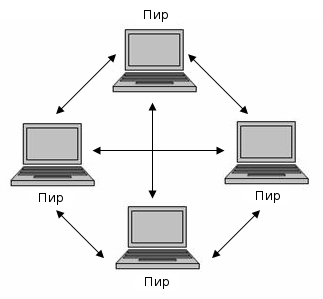
\includegraphics[width=0.6\linewidth]{peer}}
\caption{Организация peer-to-peer сети}
\label{0:peer}
\end{figure}

При работе в рамках парадигмы Peer-to-Peer (сокращенно P2P) компьютеры обмениваются ресурсами непосредственно друг с другом, без использования центрального сервера. Подход P2P обеспечивает решение проблем, возникших в результате экспоненциального роста интернет-сетей и веб-контента. Применение P2P позволило множеству польователей, которые раньше были простыми потребителями информации, поучаствовать в ее предоставлении. В момент своего появления P2P было скорее модным словом, чем продуманной концепцией. В результате мощного продвижения, в том числе, с помощью средств массовой информации, технология P2P распространилась в академических и промышленных кругах.

Основные достоинства одноранговых (Peer-to-peer) вычислительных систем:
\begin{itemize}
\item упрощается поддержка масштабируемости при значительном росте количества узлов в вычислительной сети; 
\item повышается отказоустойчивость сети, т.к. сбой любого вычислительного узла не может привести к остановке функционирования сети в целом.
\end{itemize}

Тем не менее, существует ряд препятствий при построении P2P сетей:
\begin{itemize}
\item при работе с P2P приложениями, вычислительный узел берет на себя функции как клиента, так и сервера. Это приводит к увеличению требований к производительности каждого компьютера, включенного в такую сеть.
\item низкая степень защищенности машин, участвующих в P2P сети объясняется тем, что они предоставляют открытый доступ к своим ресурсам (таким как такты процессора, определенные папки на жестком диске и т.п.). Таким образом, при отсутствии средств защиты, компьютеры, включенные в P2P подвержены риску взлома или заражения со стороны недобросовестных участников. 
\item при построении P2P сети приходится преодолевать возможную гетерогенность аппаратного и программного обеспечения ее потенциальных участников. Этот вопрос может быть решен путем применения таких технологий как XML, Java и т.д.
\item Основная проблема P2P сетей~--- это поиск доступных ресурсов без использования централизованной системы управления. Каждому узлу приходится производить поиск среди сотен и тысяч ресурсов внутри сети, что является весьма трудоемкой задачей.
\end{itemize}

\paragraph{Сервис-ориентированная архитектура}
В начале 2000-х годов мировое бизнес-сообщество занялось разработкой следующего поколения спецификаций, призванных решить проблемы ранних стандартов распределенных объектных технологий посредством веб-сервисов и сервис-ориентированной архитектуры (Service-Oriented Architecture~--- SOA).

\begin{figure}[h]
\center{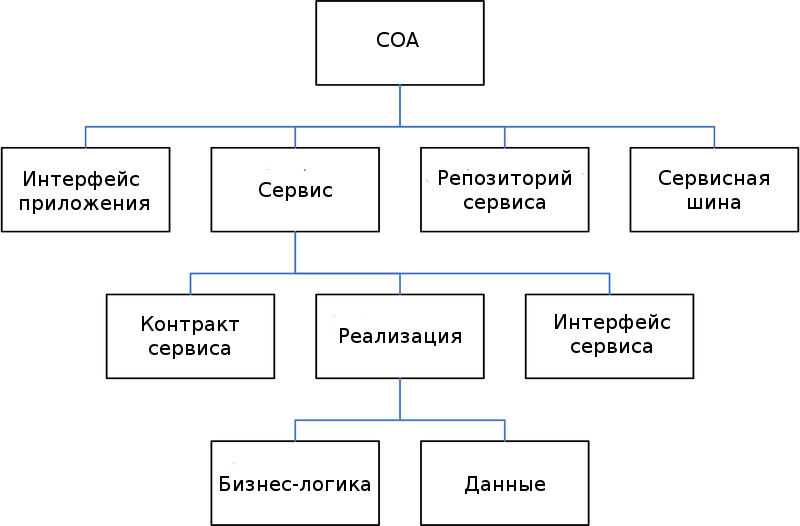
\includegraphics[width=1\linewidth]{soa}}
\caption{Одна из возможных реализаций архитектуры SOA}
\label{0:soa}
\end{figure}

Архитектура SOA не привязана к какой-либо определенной технологии. Она может быть реализована с использованием широкого спектра подходов: REST, RPC, DCOM, CORBA или веб-сервисов.

Главное, что отличает SOA~--- это использование независимых сервисов с четко определенными интерфейсами, которые для выполнения своих задач могут быть вызваны неким стандартным способом, при условии, что сервисы заранее ничего не знают о приложении, которое их вызовет, а приложение не знает, каким образом сервисы выполняют свою задачу.

SOA также может рассматриваться как стиль архитектуры информационных систем, который позволяет создавать приложения, построенные путем комбинации слабо-связанных и взаимодействующих сервисов. Эти сервисы взаимодействуют на основе какого-либо строго определенного платформо- и языко-независимого интерфейса (например, WSDL). Определение интерфейса позволяет скрывать внутреннюю реализацию сервиса.

Стандарты веб-сервисов были разработаны по инициативе организаций, занимающихся предоставлением удаленного доступа к определенным вычислительным ресурсам, и закреплены консорциумом W3C. К основным стандартам разработки и функционирования веб-сервисов можно отнести:
\begin{itemize}
\item SOAP~--- основанный на XML протокол взаимодействия веб-сервисов;
\item WSDL (Web Services Description Language~--- Язык описания веб-сервисов)~--- это методология описания ресурсов, предоставляемых веб-сервисом;
\item UDDI (Universal Description Discovery and Integration~--- Универсальный метод поиска и интеграции)~--- метод описания, поиска, взаимодействия и использования веб-сервисов. На сегодняшний день, сервис-ориентированный подход является стандартом «де-факто» при разработке распределенных вычислительных систем.
\end{itemize}

\paragraph{Программные агенты}
Несмотря на все преимущества технологии веб-сервисов, они не предоставляют новых методологий и решений построения широкомасштабных вычислительных сетей. Одним из вариантов решений, ведущихся в этом направлении, может быть рассмотрена агентно-ориентированная парадигма построения распределенных вычислительных систем. Вычислительные сети на основе так называемых программных агентов~--- это принципиально иной подход к организации систем и приложений.

Технология прогрммных агентов является основой реализации данного дипломного проекта, и будет детально рассмотрена в следующем подразделе.

\section{Концепция агентно-ориентированного программирования}
\subsection{Историческое развитие агентно-ориентированного подхода}
История теории агентов неразрывно связана с общим контекстом становления кибернетики, теории автоматов, искусственного интеллекта как научных дисциплин, моделирующих поведение искусственных и биологических сущностей в условиях некоторой внешней среды.

Фундаментальным базисом для формирования агентно-ориентированных представлений послужили труды А. Н.~Колмогорова по теории информации и алгоритмической сложности объектов, И.~Пригожина, И.~Стенгерс, Г.~Хакена по теории самоорганизации и эволюции открытых систем, У.Р.~Эшби по моделям гомеостазиса и разнообразию систем, А.~Беркса по клеточным автоматам и моделированию эволюционных систем, Дж.~Холланда и Д.~Гольдберга по генетическим алгоритмам.

Большую роль в становлении агентно-ориентированного подхода сыграли работы Карла Хьюитта в области открытых систем и теории акторов. Предложив в 1969 г. язык PLANNER для доказательства теорем, К.~Хьюитт раскрыл значение процессов коммуникации и управления в организации и понимании рассуждений. Отойдя от рассмотрения управления как последовательности актов выбора, он ввел вариант распределенной системы, в которой структуры управления трактовались как <<образцы прохождения сообщений>>, циркулирующих между активными объектами, названными им акторами. По К.~Хьюитту, актор~--- это программный агент, имеющий свой почтовый адрес и обладающий определенным поведением. В результате появилось семейство языков для программирования задач параллельного искусственного интеллекта, которые стали первыми средствами реализации мультиагентных систем, осуществляющих коммуникацию путем посылки асинхронных сообщений.

Первые западные практические разработки агентно-ориентированных систем  относятся к 70-м годам прошлого века и связаны с именами В.~Лессера и Д.~Лената. Их работы привели к созданию архитектуры «классной доски» и легли в основу многих дальнейших разработок по организации коммуникации между агентами. Исследуя проблематику автоматического понимания речи, они воспользовались метафорой <<классной доски>>, полагая, что решение проблемы обычно требует заранее незапланированных обращений к базам знаний. При этом структура управления процессом коммуникации предварительно не определена. Деятельность баз знаний связана с доставкой, модификацией и извлечением объектов с <<классной доски>>, на которой модель предметной области структурирована как пространство гипотез и решений. Специальное управляющее устройство разрешает конфликты доступа к <<классной доске>>, возникающие между агентами и неявно организует их совместную работу.

Другой тип управления взаимодействием агентов был предложен Д.~Ленатом и К.~Хьюиттом в системе PUPS, где была реализована идея решения задачи группой агентов (специалистов), именуемых <<beings>> (<<сущности>>). Эти <<сущности>> стремятся синтезировать особого специалиста по формированию концепций, способного самостоятельно решить задачу. Сами специалисты постоянно меняются в процессе решения задачи и не могут быть отнесенык классическим источникам знаний. Каждый специалист моделируется подобно фрейму множеством пар <<атрибут -- значение>> и может обращаться за сведениями к другим специалистам, не зная их лично.

В начале 80-х годов Р.~Смит разработал модель распределенного решения задач под названием «протокол контрактной сети», которая получила большую известность и стандартизована FIPA. Модель использует метафору переговоров между автономными интеллектуальными агентами и основана на протоколе рыночных торгов. Имеются три типа агентов: агент-менеджер, агент-исполнитель, агент-подрядчик. Агент-менеджер распространяет объявление о задании и определяет исходную цену, а агенты-исполнители предлагают свои услуги, посылая свои варианты цен, и участвуют в <<конкурсе>> на определение наилучших предложений по исходному заданию. Затем агент-менеджер отбирает наилучшие предложения и заключает соглашение с выбранными агентами-исполнителями, которые становятся агентами-подрядчиками.

Одной из важнейших работ начала 90-х г.г. стала статья И.~Шоэма <<Агентно-ориентированное программирование>> (АОП). В ней описан социальный взгляд на организацию вычислений, связанный с взаимодействием агентов в процессе вычислений. При этом агент рассматривается как <<прозрачный ящик>> и моделируются такие его <<внутренние переменные>> как мотивы, убеждения, обязательства, способности к выработке и принятию решений. Мотивы агента лежат в основе его решений, а убеждения определяют логические ограничения на них. Общение агентов осуществляется с помощью протоколов коммуникации.
Система АОП при таком подходе должна включать следующие базовые компоненты: ограниченный формальный язык с соответствующими синтаксисом и семантикой для описания внутреннего состояния агента; язык программирования для спецификации агентов; агентификатор, преобразующий нейтральные компоненты в программируемых агентов.

При уточнении отличий АОП от классических направлений в программировании можно опираться на представления развитые школой объектно-ориентированного программирования (ООП). Так, объект имеет имя, собственные данные и процедуры. Он может состоять из нескольких определенных объектов и в свою очередь быть частью более крупного объекта. Все действия в ООП выполняются через сообщения. В целом, понятие объекта определяется с помощью трех ключевых признаков: инкапсуляция, наследование, полиморфизм. И в отличие от объекта, агент может принять на себя определенные обязательства или, наоборот, отказаться от выполнения некоторой работы, мотивируя это отсутствием компетентности, занятостью другой задачей и т.п. В то же время, агент может выполнять такие действия как порождение, подавление и замена других агентов, активизация функций (как своих, так и у других агентов), активизация сценария деятельности, запоминание текущего состояния других агентов и пр. Все это наглядно показывает, что агент, будучи <<активным объектом>> или <<искусственным деятелем>>, формирующим свое собственное поведение, находится на более высоком уровне сложности по отношению к традиционным сущностям языков программирования.

\subsection{Агентно-ориентированный подход к программированию}
Агентно-ориентированный подход (в дальнейшем АОП) к программированию~---  разновидность представления программ или парадигма программирования, в которой основополагающими концепциями являются понятия агента и его поведение, зависящее от среды, в которой он находится. Концепция была предложена Шохемом в 1990 г. Вот определение парадигмы, данное самим автором:
"Эту новую парадигму программирования вполне разумно назвать рациональным программированием. Точно так же, как объектно-ориентированное программирование сдвинуло парадигму с написания процедур к созданию объектов, рациональное программирование сдвинуло парадигму с создания информационных объектов к созданию мотивированных агентов."

Агентный подход является следующим этапов в разработке приложений с архитектурой взаимодействующих компонентов после классического клиент-серверного подхода, позволяя сохранить его положительные черты и преодолеть большинство его недостатков. При использовании агентного подхода приложение логически делится на множество компонентов, имеющих значительную автономности и способных взаимодействовать между собой.

Использование агентов при сборе, поиске, анализе и обработке информации имеет ряд преимушеств, основные из которых сводятся к следующему:
\begin{itemize}
\item агенты могут обеспечить пользователю доступ к любым Интернет-сервисам и сетевым протоколам;
\item агент может получать и решать новые задачи, будучи уже занятым решением других задач, за счет возможности копировать себя и передавать своим копиям новые задачи;
\item агенты могут осуществлять поиск по заданию пользователя автономно, после отключения его от сети, и уведомляя о полученных результатах при следующем его подключении;
\item мобильность позволяет агентам проводить поиск (обработку) информации непосредственно по месту ее размещения, что увеличивает скорость и эффективность обработки, а также уменьшает загрузку сети;
\item агенты могут создавать собственную базу информационных ресурсов, которая может постоянно обновляться и расширяться с каждым проделанным заданием;
\item возможность агентов сотрудничать друг с другом позволяет использовать их опыт в процессе выполнения задачи;
\item агенты могут осуществлять мониторинг источников информации, уведомляя пользователя о появлении новых данных;
\item агенты могут адаптироваться под предпочтения и желания пользователя;
\item агенты могут работать с информацией, учитывая её контекст;
\item агенты могут работать с информацией интеллектуально, например, используя словари, тезаурусы, онтологии и др., а также средства вывода релевантной информации, не представленной явно ни в запросе, ни в найденных документах.
\end{itemize}

Кроме того, использование агентных технологий:
\begin{itemize}
\item упростит процессы размещения (deployment) программного обеспечения в условиях сети, автоматизируя процессы перемещения программного кода, его установки и конфигурирования;
\item упростит процессы обновления программного кода, заменяя неактивные в данный момент компоненты новыми версиями, сохраняя при этом ассоциированные с компонентом данные, совершенно прозрачно для работы всей системы в целом;
\item упростит удаленный доступ и управление в условиях сети, в том числе с использованием мобильных устройств, таких как планшетные компьютеры и сотовые телефоны;
\item значительно уменьшит сетевой трафик и общую избыточность информации за счет возможности непосредственного перемещения кода агента к обрабатываемым данным, вместо перемещения самих данных, как в случае использования клиент-серверного подхода.
\item даст возможность балансировать нагрузку между несколькими вычислительными ресурсами и вести параллельную обработку данных за счет возможности асинхронной коммуникации между агентами и возможности перемещения кода агента по сети;
\item значительно сократит время и затраты на администрирование;
\item упростит разработку программного обеспечения за счет широких возможностей повторного использования уже существующего программного обеспечения.
\end{itemize}

\subsection{Понятие агента и его свойства}
Э.~Таненбаум~--- всемирно известный специалист в области информационных технологий~--- определяет программный агент как автономный процесс, способный реагировать на среду исполнения и вызывать в ней изменения, возможно, в кооперации с пользователями или другими агентами. Таненбаум также приводит классификацию агентов, в которой выделяются следующие основные типы.
\begin{figure}[h]
\center{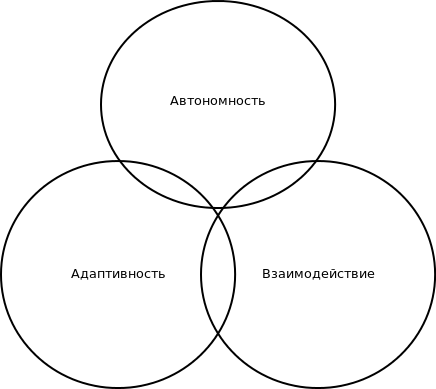
\includegraphics[width=0.6\linewidth]{tanenbaum-agent}}
\caption{Образующие свойства агента по Э.~Таненбауму}
\label{1:tanenbaum-agent}
\end{figure}

\begin{itemize}
    \item стационарные и мобильные агенты. Мобильные агенты способны перемещаться с одного узла ВС на другой. Стационарные~--- прикреплены к конкретному вычислительному узлу;

    \item кооперативные и конкурирующие. Кооперативный агент~--- способный объединяться с другими агентами для решения общей задачи. Конкурирующий~--- способен конкурировать с другими агентами с целью защиты интересов своего владельца (например, торговые агенты на бирже).
\end{itemize}

Агенты могут применяться при решении следующих задач:
\begin{itemize}
\item мобильные вычисления (миграция агентов может поддерживаться не только между постоянно подсоединенными к сети узлами, но и между мобильными платформами, подключаемыми к постоянной сети на некоторые промежутки времени и возможно по низкоскоростным каналам). Клиент подсоединяется к постоянной сети на короткий промежуток времени с мобильной платформы, отправляет агента для выполнения задачи и отсоединяется; затем клиент подсоединяется к другой точке сети и забирает результаты работы агента. Второй вариант~--- сервер, на который должен переместиться агент, подсоединяется к сети, а затем отсоединяется. В этом случае агент должен уметь переместиться на такой временно подсоединяемый сервер и вернуться в постоянную сеть;
\item задачи управления информацией:
    \begin{itemize}
    \item поиск информации (один человек не в состоянии найти необходимую ему информацию и проанализировать ее~--- использование агента, который перемещается по сети в поисках информации, может удобным образом решить подобную задачу); поисковые агенты содержат сведения о различных информационных источниках (включая тип информации, способ доступа к ней, а также такие характеристики информационного источника, как надежность и точность данных);
    \item отбор (обработка) информации. Из всех данных, приходящих к клиенту, выбирают только те данные, которые могут быть интересны клиенту. Подобный подход удобно использовать в комбинации с поисковыми агентами (сначала поиск, затем~--- отбор);
    \item мониторинг данных. Извещение пользователя об изменениях в различных источниках данных в реальном времени (например, схема, в которой мобильный агент перемещается на вычислительный узел, на котором расположен источник данных, намного эффективнее эффективнее использования статических моделей, посылающих запросы источнику данных);
    \item универсальный доступ к данным. Для чего могут быть использованы агенты–посредники, имеющие механизмы для взаимодействия друг с другом и способные работать с различными источниками данных (например, агент создает несколько других агентов, каждый из которых работает со своим источником данных).
    \end{itemize}
\end{itemize}

С.~Франклин и А.~Грэссер в 1996 году предложили следующее обобщенное определение агента: <<Автономный агент~--- это система, находящаяся внутри окружения и являющаяся его частью, воспринимающая это окружение (его сигналы) и воздействующая на окружение для выполнения собственной программы действий.>>
\begin{figure}[h]
\center{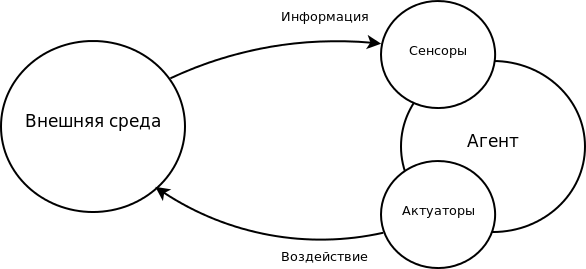
\includegraphics[width=0.8\linewidth]{franklin-agent}}
\caption{Модель автономного агента С.~Франклина и А.~Грэссера}
\label{1:franklin-agent}
\end{figure}

Можно выделить следующие основные составляющие автономного агента:
\begin{enumerate}
\item Сенсоры: блоки агента, обеспечивающие получение информации об окружающей среде и других агентах;
\item Актуаторы: блоки агента, обеспечивающие воздействие на окружающую среду.
\end{enumerate}

Автономный агент должен обладать следующими свойствами:
\begin{itemize}
\item реактивность;
\item автономность;
\item целенаправленность;
\item коммуникативность.
\end{itemize}

Свойство реактивности означает, что агент временами отвечает на изменения в окружении. Агент имеет сенсоры, с помощью которых получает информацию от окружения. Сенсоры могут быть самыми различными. Это могут быть микрофоны, воспринимающие акустические сигналы и преобразующие их в электрические, видеокарты захвата изображений, клавиатура компьютера или общая область памяти, в которую окружение помещает данные и из которой программный агент берет данные для вычислений. Не все изменения окружения становятся известными (доступными) сенсорам агента. Это вполне естественно. Ведь и человек не воспринимает звуки частотой свыше 30 кГц, радиоволны и т.д. Таким образом, окружение не является полностью наблюдаемым для агента. Аналогично, агент воздействует на окружение путем разнообразных исполнительных механизмов, включая общую память. Разумеется, степень воздействия как и степень восприятия является ограниченной. Агент может перевести окружение из некоторого состояния в некоторое другое, но не из любого в любое.

Свойство автономности означает, что агент является самоуправляющимся, сам контролирует свои действия. Программный агент, находящийся на некотором сервере, обладает возможностью <<самозапуска>>. Он не требует от пользователя каких-либо специальных действий по обеспечению его старта.

Свойство целенаправленности означает, что у агента имеется определенная цель и его поведение (воздействие на окружение) подчинено этой цели, а не является простым откликом на сигналы из окружения. Иначе говоря, агент является управляющей системой, а не управляемым объектом.

Свойство коммуникативности означает, что агент общается с другими агентами (включая людей), используя для этого некоторый язык. Это не обязательно единый язык для всех агентов. Достаточно, чтобы у пары общающихся агентов был общий язык. Язык может быть сложным как, например, естественный язык. Но может быть и примитивным: обмен числами или короткими словами.

В отдельную категорию интеллектуальных агентов выделяют автономные агенты, обладающей свойством обучаемости. Свойство обучаемости означает, что агент может корректировать свое поведение, основываясь на предыдущем опыте. Это не просто накопление в памяти параметров окружения, т.е. использование исторических данных, но сопоставление истории собственных действий с историей их влияние на окружение, и изменение в связи с этим своей программы действий.

\subsection{Агентные (мультиагентные) системы}
Мультиагентной системой (МАС) называется система, решающая одну задачу несколькими агентами методом передачи знаний и задач (действий) между агентами. Ее агенты ограничены (не знают о всей системе) и децентрализованы (не управляют всей системой).

Многоагентные системы могут быть использованы для решения таких проблем, которые сложно или невозможно решить с помощью одного агента или монолитной системы.

В таких системах необязательно все агенты взаимодействуют (общаются) между собой. В крайнем случае, общения нет вообще. Такие системы являются дискретными мультиагентными системами. Второй крайний случай~--- каждый агент общается с каждым. Такая система будет полносвязной мультиагентной системой.

Мультиагентная система, действующая как единый агент, должна характеризоваться и некоторой общей для всех субагентов целью и координацией действий по достижению этой цели.

Поскольку встречаются и другие ситуации, когда агенты не связаны столь тесно, то такие системы можно назвать обществами агентов. Отсутствие единой цели, однако, не отрицает возможного группового поведения агентов. Но оно будет являеться, скорее, эпизодическим, чем систематическим.

Еще одним возможным отличием мультиагентной системы от программы или одного агента является то, что входящие в систему программные агенты могут быть спроектированы не для какой-либо определенной системы, и таким образом составлять композицию. Может быть, это~--- повторно используемые агенты, или агенты, разработанные для решения более универсальных задач. В этих случаях агенты имеют собственные цели, не совпадающие полностью с целями системы (организации), но совместимые с ними. Тем не менее, они могут быть полезны друг другу для решения стоящих перед ними задач и, поэтому, очень важным для них с этой точки зрения является свойство коммуникативности.

С организационной точки зрения существуют общие цели всего сообщества, и эти общие цели выражаются, прежде всего, в ролях (которые играют агенты) и нормах взаимодействия.

Исследования в области систем поддержки принятия решений (DSS) в последние годы все больше переходят от создания систем в виде традиционного <<ящика с инструментами>> (toolbox) к парадигме сотрудничества и интеграции независимых приложений. Быстро растущая область исследований и нтеллектуальных агентов и мультиагентных систем предлагает возможности создания более эффективных систем на основе единого подхода.

Программирование МАС можно разделить на:
\begin{itemize}
\item составление примитивов агента;
\item организацию (архитектура и функции);
\item цели (состояние агента во времени, влияние выполнения задачи на состояние, как достигаются цели и что приосходит если их нельзя достигнуть);
\item определение окружения агентов;
\item межагентное взаимодействие.
\end{itemize}

\subsection{Стандарты агентных систем}
\begin{figure}[h]
\center{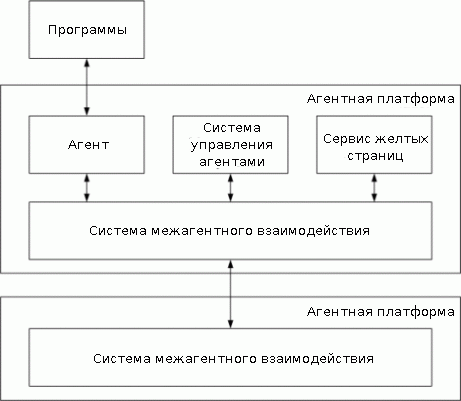
\includegraphics[width=0.6\linewidth]{fipa}}
\caption{Архитектура FIPA}
\label{1:fipa}
\end{figure}

В настоящее время ведется активная работа над разработкой стандартов, описывающих функционирование агентов и агентных систем~--- одним из ведущих является стандарт Фонда интеллектуальных программных агентов~--- FIPA.

FIPA предлагает коллекцию стандартов, направленных на продвижение гетерогенных агентов и сервисов, которые они предоставляют. Эти спецификации в общих чертах описывают коммуникационные языки агентов, услуги агентов и онтологии поддержки агентов в мультиагентных системах.

FIPA~--- является международным стандартом, который описывает функции агентных технологий, и совместимость стандартов агентов с другими технологиями. FIPA-стандарты были организованы специально для агентов и многоагентных систем и были официально приняты 8 июня 2005 года. FIPA сыграл решающую роль в развитии стандартов для агентов и их взаимодействия друг с другом, услуг, которые они могут представлять.

Стандарты FIPA включают в себя описания основных компонентов, которые должны составлять агентные системы, а также окружающую агентов среду и способы связи между собой. Также, для того чтобы облегчить связь между агентными системами разных разработчиков, FIPA-стандарты описывают стандартизированные интерфейсы, которыми должны пользоваться агенты для связи друг с другом~--- Agent Communication Language (ACL). По FIPA агенты могут обмениваться сообщениями с использованием трех протоколов~--- WAP, IIOP и  HTTP. Кроме этого, в стандартах FIPA описывается диспетчер задач и диспетчер сообщений~--- два обязательных для агентной платформы сервиса. Первый из них необходим для выбора поведений, которые агент выполняет параллельно. Второй нужен для содержания очереди сообщений.

\section{Программная среда разработки мультиагентных систем и приложений JADE}
\subsection{Общее представление и описание среды}
Java Agent Development Framework (JADE)~--- программная среда разработки мультиагентных систем и приложений, поддерживающая FIPA-стандарты для интеллектуальных агентов. Именно эта реализация технологии программных агентов для платформы Java используется в данном дипломном проекте для разработки распределенной системы.
\begin{figure}[h]
\center{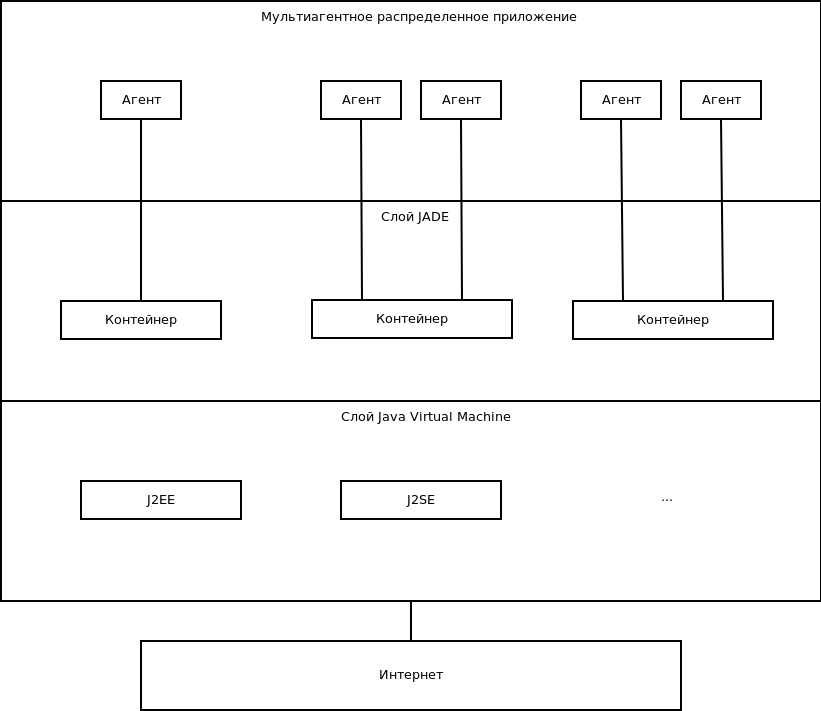
\includegraphics[width=0.8\linewidth]{fipa2}}
\caption{Мультиагентное приложение в рамках JADE}
\label{1:tanenbaum-agent}
\end{figure}

Данная платформа включает в себя:
\begin{itemize}
\item среду выполнения агентов. Агенты регистрируются и работают под управлением среды;
\item библиотеку классов, которые используются для разработки агентных систем;
\item набор графических утилит для администрирования и наблюдения за жизнедеятельностью активных агентов.
\end{itemize}

Программная среда JADE может быть подключена к любому проекту на языке Java.
JADE~--- это программное обеспечение промежуточного слоя, разработанное компанией TILAB, предназначенное для создания распределенных мультиагентных приложений на основе транспортной архитектуры <<точка -- точка>>. И интеллект, и инициатива, и информация, и ресурсы, и контроль могут быть полностью распределены по мобильным терминалам также как и по компьютерам выделенной сети. Среда может динамично взаимодействовать с узлами, которые в терминологии JADE называются агентами. Агенты то появляются, то исчезают в системе в соответствии с потребностями и требованиями программной среды.

Коммуникации между узлами не зависят от типа сети (проводная, беспроводная). Они являются полностью симметричными, и каждый узел может, как инициировать запросы, так и отвечать на них.

Платформа JADE полностью разработана на языке Java. Основополагающие принципы платформы:
\begin{itemize}
\item функциональная совместимость~--- продукт JADE разработан в соответствии со спецификациями FIPA. Как следствие JADE-агенты могут взаимодействовать со сторонними агентами, поддерживающими этот стандарт;
\item портируемость и единообразность~--- продукт JADE предоставляет гомогенный набор прикладных программных интерфейсов(API), которые не зависят ни от базового устройства сети, ни от версии платформы Java. Если подробнее, то в процессе исполнения данное ПО предоставляет одни и те же API для окружений J2EE, J2SE, J2ME. При развертывании разработчики приложений должны определить тип среды исполнения Java;
\item простота использования~--- набор простых и интуитивно-понятных интерфейсов API прячет сложную логику ПО промежуточного слоя от пользователя;
\item принцип <<разрабатывать по средствам>>~--- программистам нет необходимости использовать все возможности, которые предоставляет ПО промежуточного слоя. От программистов не требуется знать что-либо о неиспользуемых функциях платформы. Ни одна из незадействованных функций не создает дополнительные накладные вычислительные расходы.
\end{itemize}

\subsection{Контейнеры и платформы}
На рисунке \ref{2:jade} показаны основные архитектурные элементы платформы JADE.
\begin{figure}[h]
\center{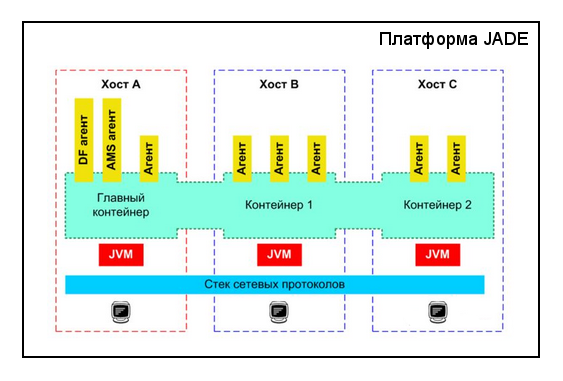
\includegraphics[width=0.9\linewidth]{jade}}
\caption{Составные части платформы JADE}
\label{2:jade}
\end{figure}

Платформа JADE состоит из системы контейнеров, распределенных в сети.
Обычно на каждом хосте находится по одному контейнеру (но для отладочных целей их может быть несколько). Агенты существуют внутри контейнеров, где обеспечиваются описанные выше системные сервисы. В системе может быть только один главный контейнер, который представляет собой точку начальной загрузки платформы. Главный контейнер создается первым, все созданные позже контейнеры должны быть зарегистрированы в главном контейнере.

Главный контейнер хранит набор системных агентов, которые обеспечивают сервисы необходимые для взаимодействия агентов:
\begin{itemize}
\item AMS (Agent Management System)~--- данный агент управляет всей платформой. Этот агент необходим для взаимодействия агентов платформы, он обеспечивает доступ агентов к сервису белых страниц платформы и управляет их жизненным циклом. AMS обеспечивает различные операции платформы, такие как: создание и удаление агентов, удаление контейнеров, завершение работы платформы. Каждому агенту необходимо зарегистрироваться в AMS, для получения персонального идентификатора AID. Запуск агента AMS происходит внутри главного контейнера платформы, но может существовать в любом контейнере. Агент, совершающий действия связанные с функционированием платформы, должен вначале запросить подтверждение у агента AMS;
\item DF (Directory Facilitator)~--- агент обеспечивает регистрацию сервисов и поиск агента по сервису в желтых страницах. Агенты платформы могут подписываться у DF-агента на получение информации о регистрации необходимого сервиса.
\end{itemize}

Внутри каждого контейнера содержится:
GADT (global agent descriptor table)~--- это регистр агентов платформы, в котором хранятся их текущий статус и местоположение.
LADT (local agent descriptor table)~--- тоже самое что и GADT, но для агентов контейнера.

\subsection{Жизненный цикл агента}
В общем случае, жизненный цикл агента включает в себя:
\begin{itemize}
\item создание агента (Agent Creation)~--- исходная точка, с которой начинается существование агента;
\item принятие решения (Making Decision)~--- основное состояние агента;
\item ожидание задания (Waiting for task)~--- состояние пассивного ожидания задания;
\item выполнение задания (Task Execution)~--- активное состояние;
\item возврат результатов (Results Return)~--- передача результатов обработки агенту-инициатору, запросившему выполнение задания;
\item делегирование задания (Delegate)~--- передача всего задания или его части одному или нескольким агентам;
\item ожидание результатов (Waiting for Results)~--- ожидание результатов обработки делегированных задач;
\item клонирование (Clone)~--- создание собственной копии, выполняющейся параллельно оригиналу;
\item перемещение (Move)~--- перемещение собственного тела на другую вычислительную платформу;
\item приостановка (Suspend)~--- временная остановка для экономии ресурсов вычислительной платформы;
\item взаимодействие со средой (Environment Interaction) – запросы к датчикам и мониторинг состояния среды;
\item уничтожение (Terminate)~--- завершающий этап жизненного цикла агента.
\end{itemize}

Такие состояния как перемещение или клонирования являются опциональными: не каждому агенту в процессе своего жизненного цикла потребуются переходы в данные состояния.

Класс Agent обеспечивает открытые методы для перехода из одного состояния в другое; эти методы получили названия от соответствующих переходов в машине конечных состояний:
\begin{itemize}
\item doActivate()~--- переводит агента из состояния AP\_SUSPENDED в состояние AP\_ACTIVE или AP\_WAITING (в зависимости от того состояния, в котором находился агент при вызове doSuspend()). doClone(Location, String) - переводит агента в состояние AP\_COPY из AP\_ACTIVE;
\item doDelete()~--- переводит агента из состояний AP\_SUSPENDED, AP\_WAITING, AP\_ACTIVE в состояние AP DELETED;
\item doMove(Location)~--- переводит агента из состояния AP\_ACTIVE в состояние AP\_TRANSIT;
\item doSuspend()~--- переводит агента из состояний AP\_ACTIVE или AP\_WAITING в состояние AP\_SUSPENDED. Состояние будет сохранено и восстановлено при вызове метода doActivate();
\item doWait(), doWait(long)~--- переводит агента из состояния AP\_ACTIVE в состояние AP\_WAITING;
\item doWake()~--- переводит агента из состояния AP\_WAITING в состояние AP\_ACTIVE.
\end{itemize}

\begin{figure}[h]
\center{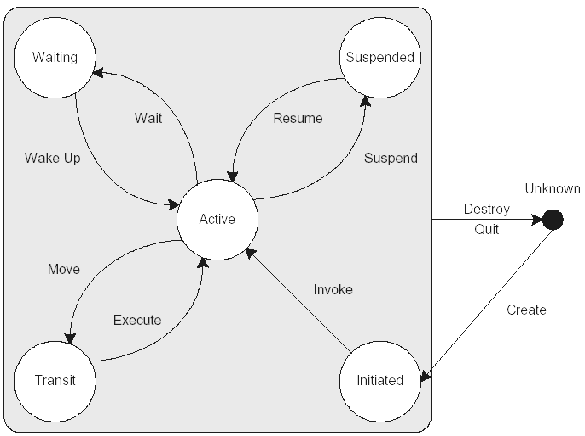
\includegraphics[width=0.8\linewidth]{life-cycle}}
\caption{Диаграмма состояний жизненного цикла агента}
\label{2:life-cycle}
\end{figure}

Агент выполняет поведения (задачи) только в состоянии AP\_ACTIVE. При вызове метода doWait() блокируется целиком весь агент и вся его деятельность, а не выполняемые правила поведения, откуда был произведен вызов данного метода. Для блокирования выполняемого поведения применяется метод block(), который переводит его в спящий режим.

\subsection{Поведение агента}
Для отработки реакции на события агент имеет поведения. Агент может отрабатывать несколько поведений одновременно. Обработка поведений происходит не по приоритетам (как Java потоки), а совместно. Очередность исполнения отдельных простых поведений не гарантируется, для этого нужно использовать поведения специальных типов или синхронизацию.
Поведениям не выделяются отдельные потоки, так как при большом количестве поведений происходит постоянное переключение между ними, а переключение между потоками происходит относительно долго (вызов поведения как метода происходит в среднем в 100 раз быстрее, чем переключение потоков).
\begin{figure}[h!]
\center{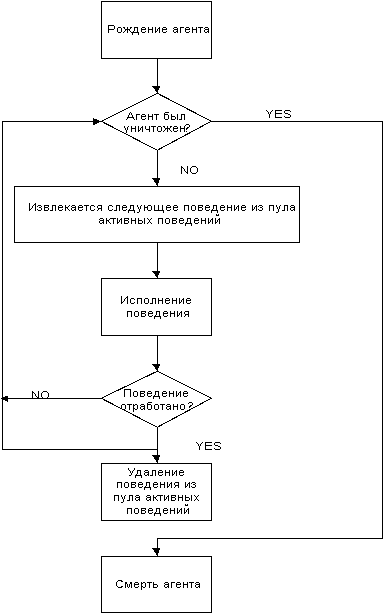
\includegraphics[width=0.6\linewidth]{behs}}
\caption{Алгоритм работы поведений агента}
\label{2:behs}
\end{figure}
В JADE можно выделить три типа поведения.
<<Единоразовое>> поведение. Данный тип поведения завершается сразу, и его метод action() выполняется только один раз. jade.core.behaviours.OneShotBehaviour уже реализовывает метод done(), возвращая true, и может быть удобным образом пронаследован, для реализации данного типа поведения.
\begin{verbatim}
public class  MyOneShotBehaviour extends OneShotBehaviour { 
   public void action() { 
       // perform operation X 
   } 
 }
\end{verbatim}
В данном примере операция X выполнится один раз.

<<Циклическое>> поведение никогда не завершается, и его метод action() выполняет одни и те же операции при каждом вызове. jade.core.behaviours.CyclicBehaviour уже реализовывает метод done(), всегда возвращая false, и может быть пронаследован для реализации циклических моделей поведения.
\begin{verbatim}
public class  MyCyclicBehaviour extends CyclicBehaviour { 
   public void action() { 
       // perform operation Y 
   } 
}
\end{verbatim}
Операция Y будет выполняться в цикле бесконечно (пока агент, имеющий это поведение, не будет завершен).

Общий случай поведения включает в себя статус, в зависимости от которого выполняются различные операции. Выполнение действий завершается, когда встречается данное условие.
\begin{verbatim}
public  class MyThreeStepBehaviour extends Behaviour { 
   private int step = 0; 
   public void action() { 
       switch (step) { 
           case 0: 
           // perform operation X 
           step++; 
           break; 
           case 1: 
           // perform operation Y 
           step++; 
           break; 
           case 2: 
           // perform operation Z 
           step++; 
           break; 
       } 
    } 

    public boolean done() { 
        return step == 3; 
    } 
}
\end{verbatim}
Jade предоставляет возможность соединять простые формы поведения для создания более сложных (SequentialBehaviour, ParallelBehaviour и FSMBehaviour). Помимо этого, Jade содержит два готовых класса (в пакете jade.core.behaviours), с помощью которых можно легко реализовать поведение, позволяющее выполнять определённые действия в заданные моменты времени.
\begin{itemize}
\item WakerBehaviour, в котором методы action() и done() уже реализованы таким образом, что вызывается абстрактный метод handleElapsedTimeout() после того, как истечет заданный промежутка времени (указанный в конструкторе);
\begin{verbatim}
public class  MyAgent extends Agent { 
   protected void setup() { 
       System.out.println(“Adding waker  behaviour”); 
       addBehaviour(new WakerBehaviour(this,  10000) { 
           protected void handleElapsedTimeout() { 
               // perform operation X 
           } 
       }); 
   } 
}
\end{verbatim}
В данном случае операция X выполнится через 10 секунд после того, как будет выведена надпись <<Adding waker behaviour>>.
\item В TickerBehaviour методы action() и done() реализованы таким образом, что вызывают циклически абстрактный метод onTick(), ожидая некоторое (заданное в конструкторе) время после каждого выполнения. TickerBehaviour никогда не завершится. 
\begin{verbatim}
public class  MyAgent extends Agent { 
   protected void setup() { 
       addBehaviour(new TickerBehaviour(this,  10000) { 
           protected void onTick() { 
               // perform operation Y 
           } 
       }); 
   } 
}
\end{verbatim}
Операция Y будет выполняться с периодом в 10 секунд.
\end{itemize}

\subsection{Коммуникационные модели, язык ACL}
Коммуникационная модель, определяет то, каким образом удалённые части программы совместно работают над запросом пользователя. Наиболее распространённым подходом здесь считается пересылка сообщений, позволяющая достичь более высокой степени автономности между частями программы, чем если бы они вызывались директивно посредством RPC (Удалённого Запуска Процессов). Пересылка сообщений является концепцией, естественно подходящей агентным системам, поскольку в рамках неё агент становится чем-то достаточно независимым, как бы делающим своё и только своё дело, и лишь иногда отвечающим на запросы других агентов или самостоятельно делающим запросы, если это потребуется для его работы. В рамках этой концепции были выделены следующие модели коммуникации между агентами:
\begin{itemize}
\item Синхронная Коммуникация. Обычно, когда клиент запускает метод на сервере, сервер выполняет запрошенный метод и возвращает результат клиенту, который продолжает свою работу. Этот стиль называется синхронным, потому что клиент блокируется до тех пор, пока результаты метода не будут возвращены;
\item Асинхронная Коммуникация. При использовании асинхронной коммуникации клиенту нет необходимости ждать, пока сервер выполнит метод, вместо этого клиент продолжает выполнять свою собственную задачу. В таком случае у клиента есть несколько возможностей получить результаты запущенного метода. Он может периодически опрашивать сервер о том, было ли закончено выполнение метода, он может ждать результата в тех случаях, когда это нужно или подписаться на уведомление о том, что результат будет доступен;
\item Динамическая Коммуникация. Этот механизм удобен в том случае, когда у клиента нет доступа к прокси серверу. Клиент может сконструировать сообщение динамически, путём указания сигнатуры того серверного метода, который должен быть запущен. Динамическая генерация сообщений может быть использована как синхронно, так и асинхронно;
\item Многосвязная Коммуникация. Многосвязная коммуникация позволяет клиентам использовать параллелизм в процессе общения с серверными объектами. Используя механизм многосвязной коммуникации, клиент может запускать один и тот же метод на нескольких серверах параллельно.
\end{itemize}
Современная система доступа к распределённым информационным ресурсам, работающая в онлайн-режиме в Internet, должна быть готова к приёму и обработке нескольких различных запросов одновременно, поэтому нельзя допустить, чтобы прохождение запросов задерживалось, пока такая система обрабатывает другой запрос. Поэтому коммуникацию между системными агентами в такой распределённой системе целесообразно организовывать по асинхронному принципу, с ориентацией на создание многопоточных программ. Однако, при создании агентов, отвечающих за работу с конечным пользователем системы, могут быть применены разные подходы.

Сервис обмена сообщениями одна из основополагающих частей архитектуры платформы JADE. Сервис основан на асинхронной передаче сообщений. Каждый агент имеет свой <<почтовый ящик>>~--- очередь входящих сообщений, куда помещаются все направленные агенту сообщения. В тот момент, когда сообщение помещается в очередь входящих сообщений, агент оповещается об этом.
\begin{figure}[h]
\center{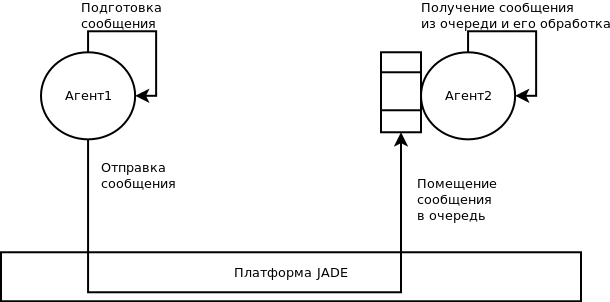
\includegraphics[width=0.6\linewidth]{acl}}
\caption{Межагентное взаимодействие в рамках платформы JADE}
\label{2:acl}
\end{figure}
Сообщения, которыми обмениваются JADE агенты имеют языковой формат ACL определенный FIPA~--- международным стандартом взаимодействия агентов. Этот формат сообщения включает в себя несколько обязательных полей и, в частности:
\begin{itemize}
\item отправитель сообщения;
\item список получателей;
\item цель общения (также называемая <<Перформативная>>), указывающая на то, что отправитель намерен достичь путем отправки сообщения. Целевыми сообщениями могут быть REQUEST (запрос), если отправитель желает, чтобы получатель совершил определенное действие, INFORM (информирование), если отправитель желает, чтобы получатель знал о некотором факте, QUERY\_IF (условный запрос), если отправитель хочет знать сохраняются ли данные условия, CFP, PROPOSE(предложение), ACCEPT\_PROPOSAL(принятие предложения), REJECT\_PROPOSAL(отмена предложения), если отправитель и получатель участвуют в переговорах, и многое другое; 
\item содержание т.е. фактическая информация, содержащаяся в сообщении (т.е. действия, которые будут выполняться в REQUEST сообщении, то, что отправитель желает раскрыть в INFORM сообщение ...);
\item язык содержания, т.е. какой синтаксис используется, чтобы выразить содержание (как отправителю, так и получателю необходимо иметь возможность кодировать / раскодировать выражения);
\item онтология, то есть словарь символов, используемых в их содержании и их значения(как отправитель так и получатель должны приписывать тот же смысл символам в сообщении , чтобы корректно понимать его);
\item некоторые поля, используемые для контроля нескольких одновременных разговоров и указания таймаутов для получения ответов, таких, как conversation-ID, reply-with, in-reply-to, reply-by. 
\end{itemize}
С сообщением в JADE работают как с объектом класса jade.lang.acl.ACLMessage, который имеет get и set методы обработки всех полей сообщения.

В случае межплатформенного сценария взаимодействие осуществляется по ACC (Agent Communication Channel). Контейнеры могут быть запущены с различными типами MTP, при этом ACC должен обеспечивать взаимодействие между ними.
В связи с тем, что агенты, обменивающиеся сообщениями, могут находиться как в одном, так и в разных контейнерах JADE использует два типа протокола: MTP (message transport protocol) и IMTP (internal message transport protocol).

В том случае если агенты находятся в разных контейнерах, используется RMI (Java Remote Method Invocation).

В JADE доступны различные типы протоколов MTP, такие как:
\begin{itemize}
\item CORBA IIOP MTP, основанный на стандартном Sun ORB;
\item CORBA IIOP MTP, основанный на ORBACUS и HTTP.
\end{itemize}

\section{Описание и разработка распределенной системы доступа к базам данных на основе программных агентов платформы JADE}
\subsection{Краткое описание разрабатываемой системы}
Описываемая распределенная система разрабатывалась на объектно-ориентированном языке программирования Java. Ядром системы является программная платформа JADE, включающая в себя как набор классов для реализации агентно-ориентированных приложений, так и инструментарий для запуска, управления и настройки платформ, контейнеров и агентов.

	Для хранения данных используется свободная объектно-ориентированная система управления базами данных Postgresql. В качестве библиотеки с базой используется jdbc-драйвер. Взаимодействие системы с пользователем осуществляется с помощью стандартного графического оконного интерфейса на основе средств, представляемых библиотекой Swing.

	Управление процессом разработки осуществляется с помощью системы контроля версий GIT. Это позволяет контролировать все изменения в проекте, фиксировать контрольные точки и этапы разработки, а также мгновенно переключаться между ними. Исходный код проекта синхронизируется с сервером github.com. Это позволяет иметь доступ к проекту из любого места, где есть доступ к сети интернет.

	Сборка проекта, поиск и установка зависимостей осущестляется с помощью фреймворка Maven. Это позволяет в значительной мере сократить сроки и усилия по развертыванию, переносу, изменению конфигурации проекта и другим подобным операциям.

	Проектируемая распределенная система будет состоять из наборов взаимодействующих между собой программных агентов, часть из которых будет находиться на локальном контейнере платформы и обрабатывать пользовательские  запросы к базе, а часть~--- на удаленных контейнерах, имеющих в своем составе сервер базы данных, отвечая за обработку запросов от локальных агентов-клиентов, передачу этих запросов в СУБД, обработку и передачу ответа. Пользователь, взаимодействуя с графическим интерфейсом, будет формировать запросы, отправляемые первоначально на агент-контроллер, отвечающий за логику  межагентного взаимодействия, и получать ответы от удаленных серверов в главном окне программы.
\begin{figure}[h]
\center{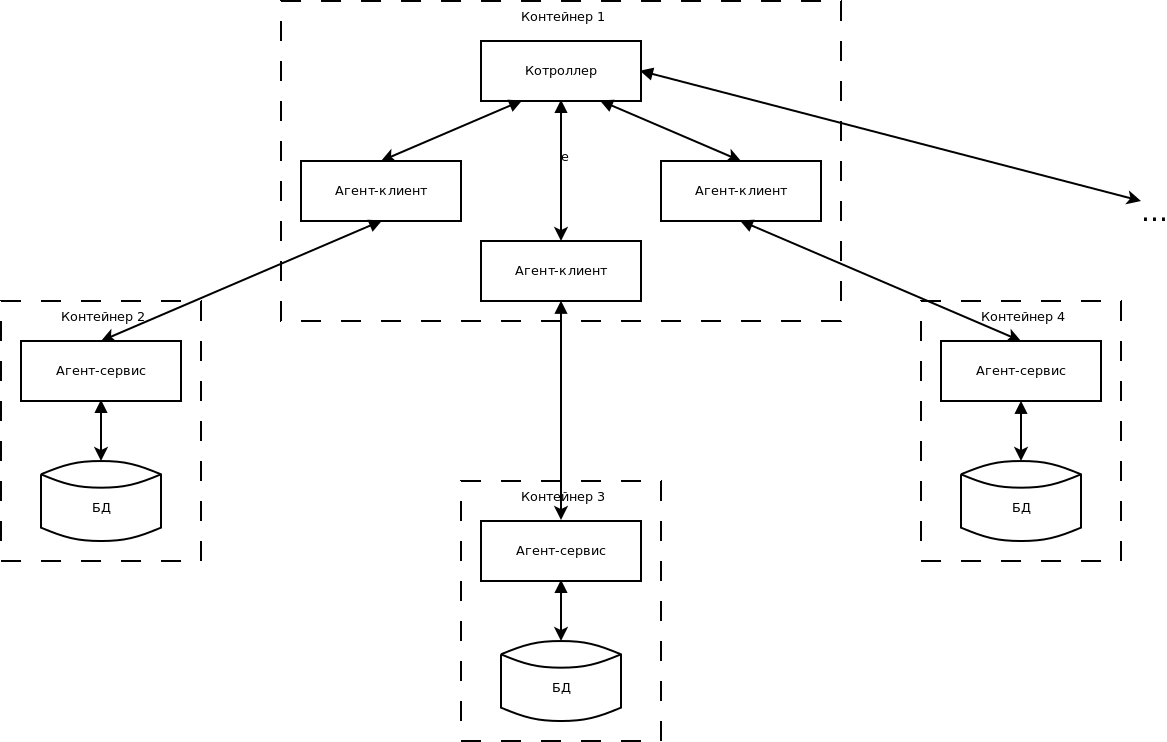
\includegraphics[width=0.9\linewidth]{common-scheme}}
\caption{Общая структура разрабатываемого приложения}
\label{3:common-scheme}
\end{figure}
Кроме этого, следует отметить, что изначально система запускается на локальном контейнере, а затем с помощью технологии мобильных агентов перемещает агенты-сервисы на имеющиеся в составе платформы удаленные контейнеры. Это позволяет иметь полную независимость от конфигураций серверных машин, версий и взаимной совместимости сервисной части системы на каждом удаленном узле. Более того, не потребуется помощь технического специалиста по настройке системы на каждом узле, не потребуется помощь и при масштабировании системы. Приложению достаточно увидеть новый контейнер в составе системы (ествественно, имеющей в своем составе необходимые для функционирования системы зависимости: JADE-платформа, без которой в общем-то и невозможно взаимное обнаружение и взаимодействие контейнеров внутри платформы, СУБД postgresql и т.д.), после чего, по указанию пользователя, будет произведена загрузка агента-сервиса на удаленный контейнер и его дальнейшее функционирование в рамках распределенной системы.

	Ниже приведена диаграмма последовательности запуска приложения и добавления нового узла (контейнера) в состав распределенной системы. Подобная последовательность событий и действий является аналогичной (начиная с события регистрации нового контейнера) при добавлении новых узлов в состав системы.
\begin{figure}[h]
\center{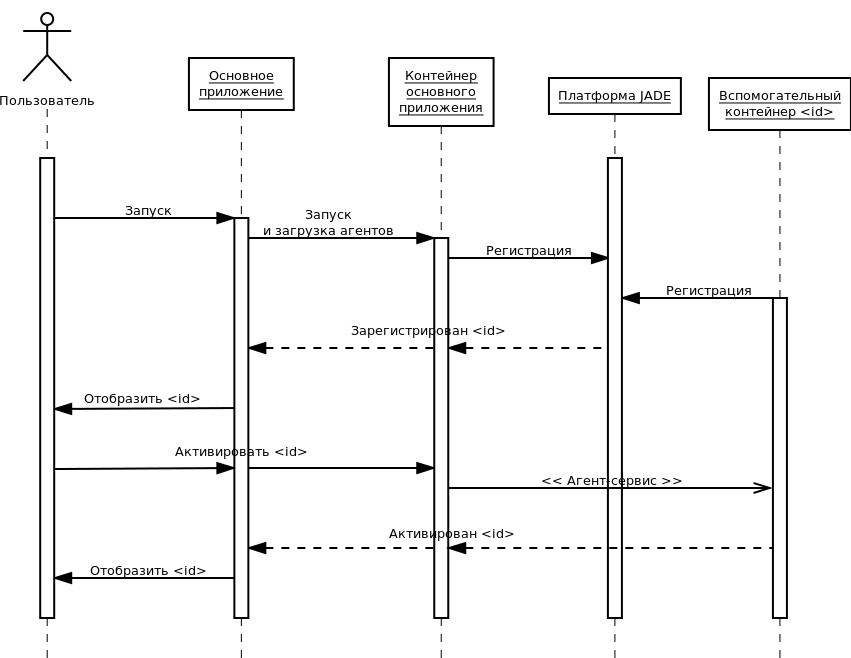
\includegraphics[width=0.9\linewidth]{seq-launch}}
\caption{Диаграмма последовательности запуска приложения и добавления нового узла}
\label{3:seq-launch}
\end{figure}
После загрузки агента-сервиса на удаленный контейнер происходит уведомление агента-контроллера, расположенного в составе модуля управления и  межагентного взаимодействия, после чего для агента-сервиса создается агент-клиент, который впоследствии будет уже напрямую обращаться к данному сервису.

Выбирая активные платформы, пользователь может обмениваться с ними информацией, не заботясь об их конфигурациях и местоположении.

Из доступных операций пользователю предоставляется возможность:
\begin{itemize}
\item получать список таблиц, расположенных на удаленном контейнере;
\item отображать контент выбранной таблицы контейнера;
\item редактировать данные выбранной таблицы;
\item добавлять данные в выбранную таблицу;
\item добавлять данные в выбранную таблицу с автоматическим реплицированием на активные контейнеры при наличии на них этой же таблицы;
\item выполнять RAWSQL-запросы на выбранный контейнер;
\item выполнять RAWSQL-запросы на все активные контейнеры.
\end{itemize}

\subsection{Описание состава пакетов системы}
\subsubsection{Состав пакета client}
Данный пакет содержит классы, входящие в состав агента-клиента. Основной класс ClientAgent, как видно из названия, реализует логику работы самого агента.

\paragraph{Класс ClientAgent}
Класс агента, как правило реализует основной метод setup(), в котором происходит инициализация агента, добавление поведений и другие операции, связанные с функционированием агента.
Ниже показано содержимое метода setup() класса ClientAgent:
\begin{verbatim}
protected void setup() {
    setEnabledO2ACommunication(true, 0);
    Object[] args = getArguments();

    switch(args.length) {
        case 3:
            serviceAID = (AID) args[2];
        case 2:
            agentInterface = (AgentInterface) args[1];
        case 1:
            ConditionalVariable startUpLatch = (ConditionalVariable) args[0];
            startUpLatch.signal();
    }

    ((AgentEvents) agentInterface).onEvent(new AID(getName(), AID.ISLOCALNAME), AgentEvents.EVENT_CLIENT_READY);
    addBehaviour(new O2ABehaviour());
}
\end{verbatim}
По-сути, содержимое метода отвечает за настройку приема данных от внешних классов, не являющихся агентами. Это реализовано с помощью технологии Object2Agent communication. Для этого необходимо включить поддержку взаимодействия O2A методом setEnabledO2ACommunication().

Далее, в контрукции switch() происходит выборка доступных аргументов, с которыми был запущен агент.

Первым аргументом (порядок аргументов идет с конца) передается мьютекс ConditionalVariable, который позволяет внешнему окружению дождаться запуска и инициализации агента. В противном случае, данные агентом получены не будут.

Второй аргумент хранит подписчика на события агента. Интерфейс AgentInterface имеет два интерфейса-потомка: AgentData и AgentEvents. Первый из них отвечает за уведомление о поступающих от агента данных, а второй~--- о возникающих событиях. В данном случае, агент посылает событие EVENT\_CLIENT\_READY, означающее готовность агента к функционированию.

Третий аргумент хранит AID~--- идентификатор~--- агента-сервиса, за которым <<закреплен>> данный агент-клиент.

В конце метода происходит добавление поведения O2ABehaviour, которое обрабатывает входящие данные от внешних модулей приложения.

\paragraph{Класс ClientBehaviour}
Основным методом объектов класса Behaviour является метод action(). Данный метод вызывается платформой по правилам, заложенным в реализации класса.

\begin{verbatim}
public void action() {
    ACLMessage message = null;

    switch (state) {
        case SENDING:
            message = new ACLMessage(ACLMessage.REQUEST);
            message.addReceiver(aid);

            try {
                message.setContentObject(agentDataContainer);
            } catch (IOException e) {
                e.printStackTrace();
            }

            myAgent.send(message);
            state++;
            break;
        case RECEIVING:
            message = myAgent.receive();
            if(message != null) {
                try {
                    agentDataContainer = (AgentDataContainer) message.getContentObject();
                } catch (UnreadableException e) {
                    e.printStackTrace();
                }

                AgentData agentData = (AgentData) ((ClientAgent) myAgent).getAgentInterface();
                AID aid = new AID(myAgent.getName(), AID.ISLOCALNAME);
                agentData.onData(aid, agentDataContainer);
                done = true;
            } else {
                block();
            }

            break;
    }
}
\end{verbatim}
Функционирование основного поведения агента-клиента реализовано в виде <<машины состояний>>. На первом этапе поведение функционирует в состоянии отправки запроса агенту сервиса, для чего формируется соотвестствующее ACL сообщение. На втором~--- в ожидании ответа от сервиса. В конце выполнения поведения происходит уведомление агента о полученных данных от агента-сервиса.

\paragraph{Класс O2ABehaviour}
Класс O2ABehaviour содержит циклический опрос очереди O2A-сообщений. При отсутствии сообщений поведение блокируется методом block() до появления нового сообщения в очереди.
\begin{verbatim}
public void action() {
    AgentDataContainer agentDataContainer = (AgentDataContainer) myAgent.getO2AObject();
    if(agentDataContainer != null) {
        myAgent.addBehaviour(new ClientBehaviour(myAgent, agentDataContainer));
    } else {
        block();
    }
}
\end{verbatim}

\subsubsection{Состав пакета service}
\paragraph{Класс ServiceAgent}
Основной класс пакета service~--- ServiceAgent. Его метод setup() аналогичен содержимому метода класса ClientAgent. Помимо этого, класс ServiceAgent реализует методы beforeMove() и afterMove()~--- это callback-методы, вызываемые платформой JADE, соотвественно до и после операции перемещения агента. Метод beforeMove() не содержит функциональной логики, а служит лишь для печати отладочной информации на консоль. Метод afterMove() добавляет новое поведение в состав агента, и посылает сообщение агенту-контроллеру о своем перемещении.
\begin{verbatim}
protected void afterMove() {
    addBehaviour(new ServiceBehaviour(this));

    System.out.println("After move: " + here());
    ACLMessage msg = new ACLMessage(ACLMessage.INFORM);
    msg.setConversationId(ControllerAgent.CONTROLLER_AGENT_CONVERSATION_ID);
    AID dest = new AID(ContainerHoldersManager.CONTROLLER_AGENT_NAME, AID.ISLOCALNAME);
    msg.setContent(getName());
    try {
        msg.setContentObject(here());
    } catch (IOException e) {
        e.printStackTrace();
    }
    msg.addReceiver(dest);
    send(msg);
}
\end{verbatim}
\paragraph{Класс ServiceAgent}
Поведение агента-сервиса ServiceBehaviour содержит интерфейсы взаимодействия с базой данных узла посредством классов, предоставляемых пакетом db. Логически поведение разбито на две части: это обработка запроса с передачей его к СУБД и формирование и отправка ответа агенту-клиенту. Кроме этого, при получении сообщения с типом CANCEL сервис завершает свою работу.
\begin{verbatim}
public void action() {
    ACLMessage msg = myAgent.receive();
    if (msg != null) {
        switch (msg.getPerformative()) {
            case ACLMessage.REQUEST:
                ACLMessage reply = msg.createReply();
                reply.setPerformative(ACLMessage.INFORM);
                AgentDataContainer agentDataContainer = null;

                try {
                    agentDataContainer = (AgentDataContainer) msg.getContentObject();
                    System.out.print(agentDataContainer);
                } catch (UnreadableException e) {
                    e.printStackTrace();
                }

                agentDataContainer = dbw.execute(agentDataContainer);
                agentDataContainer.setParam(AgentDataContainer.KEY_CONTAINER_NAME, myAgent.here().getName());

                try {
                    reply.setContentObject(agentDataContainer);
                } catch (IOException e) {
                    e.printStackTrace();
                }

                myAgent.send(reply);
                break;
            case ACLMessage.CANCEL:
                myAgent.doDelete();
                break;
        }
    } else {
        block();
    }
}
\end{verbatim}

\subsubsection{Состав пакета ctrl}
Пакет ctrl включает в себя классы, осуществляющие организацию межагентного взаимодействия, управление контейнерами, входящими в состав платформы, уведомление внешних внеагентных компонентов о событиях внутри платформы.
\paragraph{Класс ControllerAgent}
Запускает поведение мониторинка контейнеров платформы.

Уведомляет основной программный контроллер ContainerHolderManager о процедуре перемещения агентов-сервисов.

\paragraph{Класс AMSListenerBahaviour}
Данное поведение регистрирует обработчик в плтаформе JADE. Внутри обработчика добавления новых контейнеров просходит получение идентификатора контейнера и передача его контроллеру приложения.
\begin{verbatim}
public class AMSListenerBehaviour extends AMSSubscriber {
    public void installHandlers(Map handlersTable) {
        handlersTable.put(AddedContainer.NAME, new AddedContainerHandler());
    }

    public final class AddedContainerHandler implements EventHandler {
        public void handle(Event ev) {
            AddedContainer event = (AddedContainer) ev;
            ContainerID addedContainer = event.getContainer();

            ContainerHoldersManager.onContainerAdded(addedContainer);
        }
    }
}
\end{verbatim}

\paragraph{Класс ContainerHolder}
Данный класс хранит всю информацию, относящующся к конкретному контейнеру, а также предоставляет все интерфейсы для взаимодействия агентов клиента и сервиса внешним компонентам приложения. Основые поля класса:

\begin{itemize}
\item AgentController client~--- агент-клиент, относящийся к данному контейнеру;
\item AID serviceID~--- идентификатор сервиса, который расположен на данному конейнеру;
\item ContainerID containerID~--- идентификатор контейнера;
\item isActive~--- флаг активности контейнера~--- активный контейнер имеет в своем составе запущенные агенты сервиса и клиента, относящиеся к данному контейнеру.
\end{itemize}

\begin{itemize}
\item doActivate()~--- активирует данный контейнер;
\item doExecute()~--- отправляет запрос на сервис. В качестве параметра передается объект класса AgentDataContainer;
\item onData()~--- callback-функция получения информации от сервиса;
\item onEvent()~--- callback-функция получения событий от сервиса.
\end{itemize}

\paragraph{Класс ContainerHoldersManager}
Класс ContainerHoldersManager служит для организации системы распределенных узлов. В нем хранится список доступных на платфрме контейнеров, а также создает системный контейнер и запускает агента-контроллера. Помимо этого, он занимается обработкой событий, поступающих от объектов класса ContainerHolder и, в свою очередь, делегирует эти события собственным подписчикам (listeners).

\subsubsection{Пакет db}
Данный пакет состоит лишь из одного класса: DBWorker, который отвечает за всю логику взаимодействия с базами данных. Основным методом данного класса является метод execute(), который, как видно из названия выполняет запрос к базе и обрабатывает полученный ответ для выдачи результата запрашиваемому агенту-сервису.
\begin{verbatim}
public AgentDataContainer execute(AgentDataContainer agentDataContainer) {
    ...
    String dataType = AgentDataContainer.VALUE_DATA_TYPE_TABLES;

    connection = DriverManager.getConnection(url, user, password);

    if (agentDataContainer.getParam(KEY_REQUEST_STRING).equals(GET_TABLES_LIST)) {
        resultSet = connection.getMetaData().getTables(null, "public", "%", new String[]{"TABLE"});
    } else if (agentDataContainer.getDataLength() > 0) {
        boolean verified = verify(connection, agentDataContainer);
        if(verified) {
            dataType = AgentDataContainer.VALUE_DATA_TYPE_EMPTY;
            pst = connection.prepareStatement(agentDataContainer.getParam(KEY_REQUEST_STRING));

            Object[] dataRow = agentDataContainer.getData().get(0);
            for (int i = 0; i < agentDataContainer.getDataWidth(); i++) {
                pst.setObject(i + 1, dataRow[i], agentDataContainer.getMetadata()[i].getType());
            }

            pst.executeUpdate();
        }

        resultSet = null;
    } else {
        dataType = AgentDataContainer.VALUE_DATA_TYPE_CONTENT;
        pst = connection.prepareStatement(agentDataContainer.getParam(KEY_REQUEST_STRING));

        resultSet = pst.executeQuery();
    }

    outputAgentDataContainer = ResponseMaker.makeResponse(resultSet, agentDataContainer);
    outputAgentDataContainer.setParam(KEY_DATA_TYPE, dataType);
    ...
    return agentDataContainer;
}
\end{verbatim}
В ветвлении if происходит определение типа входящего запроса:
\begin{itemize}
\item получение списка таблиц;
\item операция модификации/добавления данных в таблице;
\item операция получения данных из таблицы / RAW-SQL запрос.
\end{itemize}
Кроме того, в этом методе происходит верификация корректности запроса при обращении к таблицам: это необходимо для операций репликации на всех активных узлах.

Соединение создается в строке connection = DriverManager.getConnection(). Класс DriverManager заведует драйверами, соединениями, а также трассировкой. В данном случае вызывается статический метод getConnection(). Этот метод просматривает список драйверов и, если находит подходящий к указанному URL, то создает и возвращает соединение. В противном случае выбрасывает исключение с текстом: "No suitable driver found". В качестве аргументов данный метод принимает URL к базе, имя и пароль пользователя.

Запрос для исполнения формирутеся с помощью метода prepareStatement() класса Connection. Запрос может состоять как из одной лишь текстовой строки, так и содержать объекты-параметры. Первая задается непостредственно в аргуенте метода, а последние~--- добавляться в запрос методов setObject(). Исполнение производится методом executeQuery(), либо executeUpdate() для выполнения операций вставки и модификаций в базе.

Ниже представлена архитектура JDBC, в рамках которой взаимодействует и базой данный, в том числе, и данное приложение, используя JDBC server.
\begin{figure}[h]
\center{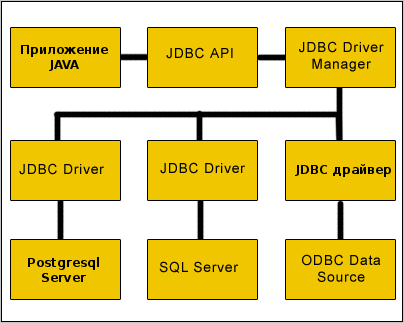
\includegraphics[width=0.7\linewidth]{jdbc}}
\caption{Взаимодействие Java-проложения с сервером БД}
\label{3:jdbc}
\end{figure}

\subsubsection{Пакет data}
\paragraph{Класс AgentDataContainer}
Данный класс является одним из наиболее универсальным и используемых сущностей в архитектуре приложения. Он пронизвыает буквально все уровни распределенной системы: начиная от классов графического пользовательского интерфейса, заканчивая обработчиком взаимодействия с сервером базы данных на удаленном узле. Данная унификация дает существенное преимущество: до тех пор, пока архитектурный уровень приложения не нуждается в содержимом информации, передаваемой другим уровням, он никак не вмешивается в их содержимое, структуру и методы, являясь лишь промежуточным звеном в коммуникационной цепочке. Это позволяет, при необходимости, изменять, дополнять, расширять архитектуру приложения, внося минимальные исправления в состав остальных компонентов.
\begin{figure}[h]
\center{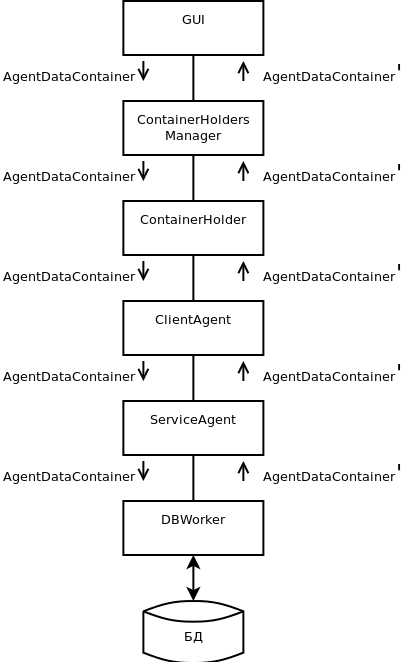
\includegraphics[width=0.5\linewidth]{comm-dia}}
\caption{Коммуникационная модель взаимодействия компонентов системы}
\label{3:comm-dia}
\end{figure}

Содержимое класса состоит из списка массива объектов, хранящих непосредственно табличные данные; массива типа <<Имя-Тип>> для хранения информации о типе и названии колонок данных; а также HashMap'a, содержащего набор <<Ключ-Значение>> для хранения таких параметров как: имя используемой таблицы, строки запроса и т.д.

\paragraph{Класс QueryMaker}
Класс QueryMaker реализует паттерн <<фабрика>> для объектов класса AgentDataContainer.

Основные методы класса:
\begin{itemize}
\item selectTables()~--- производит формирование запроса выборки списка таблиц базы;
\item selectTableContent()~--- производит выборку контента запрашиваемой таблицы;
\item insertData()~--- выполняет добавление строки данных в таблицу;
\item updateData()~--- выполняет модификацию строки данных в таблице.
\end{itemize}

\paragraph{Класс ResponseMaker}
Класс ResponseMaker выполняет сериализацию возвращаемого результа запроса к базе данных. Основной (и единственный) метод класса~--- makeResponse(). Результатом его работы является сформированный объект класса AgentDataContainer, хранящий данные, метадату и дополнительные параметры ответа: имя таблицы и хэш-код ее метадыты.
\begin{verbatim}
public static AgentDataContainer makeResponse(ResultSet resultSet, AgentDataContainer agentDataContainer) {
    NameTypePair[] metadata = null;
    List<Object[]> data = null;
    String metadataHash = "";

    if (resultSet != null) {
        try {
            ResultSetMetaData rsmd = resultSet.getMetaData();
            int columnCount = rsmd.getColumnCount();
            MetadataHasher.reset();

            metadata = new NameTypePair[columnCount];
            for (int columnIndex = 1; columnIndex <= columnCount; columnIndex++) {
                metadata[columnIndex - 1] = new NameTypePair();
                String name = rsmd.getColumnName(columnIndex);
                int type = rsmd.getColumnType(columnIndex);
                metadata[columnIndex - 1].setName(name);
                metadata[columnIndex - 1].setType(type);

                MetadataHasher.add(type, name);
            }
            metadataHash = MetadataHasher.get();

            data = new ArrayList<Object[]>();
            while (resultSet.next()) {
                Object[] row = new Object[columnCount];
                for (int columnIndex = 1; columnIndex <= columnCount; columnIndex++) {
                    row[columnIndex - 1] = resultSet.getObject(columnIndex);
                }
                data.add(row);
            }
        } catch (SQLException e) {
            e.printStackTrace();
        }
    }

    String tableName = agentDataContainer.getParam(KEY_TABLE_NAME);
    agentDataContainer = new AgentDataContainer(metadata,data);
    agentDataContainer.setParam(KEY_TABLE_NAME, tableName);
    agentDataContainer.setParam(KEY_METADATA_HASH, metadataHash);

    return agentDataContainer;
}
\end{verbatim}

\subsubsection{Пакет gui}
Набор классов данного пакета реализует графический пользовательский интерфейс приложения. Включает в себя следующие классы:
\begin{itemize}
\item ClientMainFrame~--- главное окно приложения;
\item ClientTable~--- табличный компонент для отображения данных;
\item ContainerHoldersList~--- список, отображающий доступные контейнеры платформы;
\item InsertDialog~--- модальное окно, осуществляющее добавление данных в таблицу.
\end{itemize}

\ESKDdocName{Технология автоматизированной сборки и развертывания проектов}
\updateStamp
\ESKDthisStyle{formII}
\section{Технология автоматизированной сборки и развертывания проектов с использованием фреймворка Maven}
\subsection{Концепция автоматизированной сборки программного обеспечения}
Непрерывные процессы усложнения программного обеспечения, сред и средств разработки, взаимной интеграции и использования составных частей различных технологий и приложений в одном проекте, использование методологий гибкой разработки ПО~--- зачастую делают традиционный подход к процессу ручной сборки программного обеспечения неоправнанно трудозатратным и малоэффективным.

Использование в процессе разработки систем управления версиями, таких как Git или CVS, на сегодняшний день является общепринятой практикой. Когда над одной системой работает большое число разработчиков, такая координация становится необходимой.  При этом важно быть уверенным, что последняя версия кода, находящаяся в системе управления версиями, всегда успешно собирается. Это хороший метод для проектов с замкнутыми командами разработчиков; когда разработчики периодически синхронизируют свои рабочие области с транком, несобирающийся исходный код задержит процесс разработки до исправления проблемы. Для проектов же с открытым исходным кодом сохранение основной ветки разработки в рабочем состоянии просто жизненно необходимо. Потенциальные программисты могут загрузить код в любой момент, и если он окажется в нерабочем состоянии~--- это с большой делей вероятности оттолкнет их от дальнейшего участия в таком проекте.

Другим современным аспектом разработки является подход, ориентированный на написание модульных тестов и включение их в выполнение на этапе сборки.
	Актуальная сегодня методология "экстремального программирования" (англ. Extreme Programming, XP) предполагает процесс непрерывной интеграции. Разработчики интегрируют свой код в основную ветку разработки как можно чаще~--- как правило, раз в несколько часов~--- проверяя при этом успешное выполнение всех тестов. Аналогичные методики итеративной разработки ПО придерживаются подобного подхода.

Для адаптации непрерывной интеграции и модульного тестирования необходимо, чтобы разработка проекта следовала этим методикам. Однако, зачастую этого недостаточно.

Итак, поскульку вышезложенные методы подходы состоят из неавтоматизированных шагов~--- интеграции кода, выполнения тестов и постоянном внесении кода в репозиторий~--- все это может повлечь технические трудности, излишние временные затраты и ошибки. Автоматизированная система, собирающая код и выполняющая модульные тесты, является гораздо более надежным решением.

\subsubsection{Требования к системам автоматизированной сборки ПО}
Базовые требования:
\begin{enumerate}
\item частые или <<ночные>> сборки для своевременного выявления проблем;
\item поддержка управления зависимостями исходного кода (Source Code Dependency Management);
\item обработка разностной сборки;
\item уведомление при совпадении исходного кода (после сборки) с имеющимися бинарными файлами;
\item ускорение сборки;
\item отчет о результатах компиляции и линковки.
\end{enumerate}

Дополнительные требования:
\begin{enumerate}
\item создание описания изменений (release notes) и другой сопутствующей документации (например, руководства);
\item отчет о статусе сборки;
\item отчет об успешном/неуспешном прохождении тестов;
\item суммирование добавленных/измененных/удаленных особенностей в каждой новой сборке.
\end{enumerate}

\subsubsection{Преимущества использования}
\begin{itemize}
\item улучшение качества продукта;
\item ускорение процесса компиляции и линковки;
\item избавление от излишних действий;
\item минимизация некорректных сборок;
\item избавление от привязки к конкретному человеку;
\item ведение истории сборок и релизов для разбора выпусков;
\item экономия времени и денег благодаря вышеобозначенных причинам,
\end{itemize}

\subsection{Система автоматизированной сборки Maven}
Apache Maven~--- фреймворк для автоматизации сборки проектов, специфицированных на XML-подобном языке POM (англ. Project Object Model). Maven обеспечивает декларативную сборку проекта. Это означает, что в файлах проекта pom.xml содержится его декларативное описание, а не отдельные команды. Все задачи по обработке файлов Maven выполняет через плагины.

\subsubsection{Преимущества Maven}
\begin{itemize}
\item независимость от OS. Сборка проекта происходит в любой операционной системе. При этом сборочный файл проекта остается неизменным от системы к системе;
\item управление зависимостями. Подавляющее большинство проектов пишутся с использованием сторонних библиотек (зависимостей). Эти сторонние библиотеки зачастую тоже используют другие библиотеки в качестве зависимостей. Maven позволяет управлять такими сложными процессами.  Это позволяет осуществлять поиск и установку нужного ПО, разрешать конфликты версий и, в случае необходимости, легко переходить на новые версии библиотек;
\item возможность сборки из командной строки. Такое часто необходимо для автоматической сборки проекта на сервере (практика использования подхода Continuous Integration);
\item хорошая интеграция со средами разработки. Основные среды разработки на Java без каких-либо сложностей поддерживают проекты, которые собираются c помощью фреймворка maven. При этом, зачастую, даже не требуется дополнительная настойка проекта~--- он сразу готов к дальнейшей разработке. Как следствие~--- если с проектом работают в разных средах разработки, то maven является отличным средством по унифицикации способа хранения настроек. Настроечный файл среды разработки и для сборки один и тот же~--- это уменьшает дублирование данных и, соответственно, количество ошибок;
\item декларативный стиль описания проекта. Позволяет лучшим образом формулировать конечные цели по организации проекта, не вдаваясь в детали и способы их реализации.
\end{itemize}

\subsubsection{Создание проекта под управлением maven}
Данные и последующие действия предполагают наличие установленного в системе фреймворка maven.

Для создания нового проекта необходимо ввети следующую команду:
\begin{lstlisting}
mvn archetype:generate
\end{lstlisting}
 
	Выполнив эту команду, maven покажет список шаблонов (архетипов) для разных проектов. Необходимо выбрать проект и его версию по умолчанию, Далее команда спросит groupId и artifactId.
В результате сгенерируется проект со стандартной структурой директорий:
\begin{lstlisting}
testproject1
|-- pom.xml
`-- src
    |-- main
    |   `-- java
    |       `--ru
    |           `-- ru.apache_maven
    |                   `-- App.java
    `-- test
        `-- java
            `-- ru
                `-- ru.apache_maven
                        `-- AppTest.java
\end{lstlisting}
        
В примере генерируется настройки приложения, включающего в себя помимо исходного кода набор JUnit-тестов и pom.xml~--- основной настроечный файл maven, который будет рассмотрен в следующем подразделе.

Чтобы скомпилировать код, нужно набрать в консоли: mvn compile. Успешная сборка проекта сопровождается следующим сообщением:

\begin{lstlisting}
.....
[INFO] BUILD SUCCESS
.....
\end{lstlisting}

Ввод команды “mvn package” в директории target сгенерирует jar файл testproject1-1.0-SNAPSHOT.jar.

\subsubsection{Основной файл проекта pom.xml}
pom.xml~--- это основной файл, описывающий проект. Вообще, в проекте могут использоваться дополнительные файлы, однако они играют второстепенную роль. Рассмотрим структуру файла pom.xml.

Корневой элемент и заголовок.

\begin{lstlisting}
<project xmlns="http://maven.apache.org/POM/4.0.0"
    xmlns:xsi="http://www.w3.org/2001/XMLSchema-instance"
    xsi:schemaLocation="http://maven.apache.org/POM/4.0.0
                    http://maven.apache.org/xsd/maven-4.0.0.xsd">
    <modelVersion>4.0.0</modelVersion>
    .............
</project>
\end{lstlisting}

Здесь находится корневой элемент <project>, схема, которая облегчает редактирование и проверку, и версия POM. Внутри тэга project содержится основная и обязательная информация о проекте:

\begin{lstlisting}
<!-- The Basics -->
  <groupId>...</groupId>
  <artifactId>...</artifactId>
  <version>...</version>
\end{lstlisting}

В Maven каждый проект идентифицируется парой groupId artifactId. Во избежание конфликта имен, в groupId заносится наименование организации или подразделения и обычно действуют такие же правила как и при именовании пакетов в Java~--- записывают доменное имя организации или сайта проекта. artifactId~--- название проекта. Внутри тэга version, как можно догадаться хранится версия проекта. Тройкой groupId, artifactId, version (далее~--- GAV) можно однозначно идентифицировать jar файл приложения или библиотеки. Если состояние кода для проекта не зафиксировано, то в конце к имени версии добавляется "\-SNAPSHOT"\,, что обозначает, что версия в разработке, и результирующий jar файл может меняться. <packaging>...</packaging> определяет какого типа файл будет создаваться как результат сборки. Возможные варианты pom, jar, war, ear.

Также добавляется информация, которая не используется самим мавеном, но нужна для программиста, чтобы понять, о чем этот проект:
\begin{itemize}
\item<name>powermock-core</name>~--- название проекта для человека;
\item<description>PowerMock core functionality.</description>~--- описание проекта;
\item<url>http://www.powermock.org</url>~--- сайт проекта.
\end{itemize}

\subsubsection{Зависимости}
Зависимости~--- следующая очень важная часть pom.xml~--- в данной секции хранится список всех библиотек (зависимостей) которые используюся в проекте. Каждая библиотека идентифицируется также как и сам проект~--- тройкой groupId, artifactId, version (GAV). Объявление зависимостей заключено в тэг <dependencies>...</dependencies>.

\begin{lstlisting}
<dependencies>
<dependency>
    <groupId>junit</groupId>
    <artifactId>junit</artifactId>
    <version>4.4</version>
    <scope>test</scope>
</dependency>
<dependency>
    <groupId>org.powermock</groupId>
    <artifactId>powermock-reflect</artifactId>
    <version>\${version}</version>
</dependency>
<dependency>
    <groupId>org.javassist</groupId>
    <artifactId>javassist</artifactId>
    <version>3.13.0-GA</version>
    <scope>compile</scope>
</dependency>
</dependencies>
\end{lstlisting}

Как можно заметить, кроме GAV при описании зависимости может присутствовать тэг <scope>. Scope задает спецификацию назначения данной библиотеки. В рассматриваемом примере указывается, что библиотека с GAV junit:junit:4.4 нужна только для выполнения тестов.

\subsubsection{Тэг <<build>>}
Тэг <build> является необязательным т.к. для него существуют значения по умолчанию. Этот раздел содержит информацию по самой сборке: где находятся исходные файлы, ресурсы проекта, список используемых плагинов.

\begin{lstlisting}
<build>
<outputDirectory>target2</outputDirectory>
<finalName>ROOT</finalName>
<sourceDirectory>src/java</sourceDirectory>
<resources>
    <resource>
        <directory>\${basedir}/src/java</directory>
        <includes>
        <include>**/*.properties</include>
        </includes>
    </resource>
</resources>
     <plugins>
         <plugin>
             <groupId>org.apache.maven.plugins</groupId>
             <artifactId>maven-pmd-plugin</artifactId>
             <version>2.4</version>
         </plugin>
     </plugins>
 </build>
\end{lstlisting}

Рассмотрим содержимое <build> секции.

\begin{itemize}
\item <sourceDirectory>~--- определяет, откуда maven будет брать файлы исходного кода. По умолчанию это src/main/java, но можно самостоятельно определить путь к исходному тексту. Директория может быть только одна (без использования специальных плагинов).
\item <resources> и вложенные в нее тэги <resource> определяют одну или несколько директорий, где хранятся файлы ресурсов. Ресурсы в отличии от файлов исходного кода при сборке просто копируются. Директория по умолчанию: src/main/resources 
\item <outputDirectory>~--- определяет, в какую директорию компилятор будут сохраняться результаты компиляции~--- *.class файлы. Значение по умолчанию: target/classes.
\item <finalName>~--- имя результирующего jar (war, ear..) файла с соответствующим типу расширением, который создается на фазе “package”. Значение по умолчанию: artifactId-version.
\end{itemize}

\subsubsection{Основные фазы сборки проекта}
\begin{itemize}
\item compile~--- компилирование проекта;
\item test~--- тестирование с помощью JUnit тестов;
\item package~--- создание .jar файла или war, ear в зависимости от типа проекта;
\item integration-test~--- запуск интеграционных тестов;
\item install~--- копирование .jar (war , ear) в локальный репозиторий;
\item deploy~--- публикация файла в удаленный репозиторий.
\end{itemize}

К примеру нам нужно создать jar проекта. Для его создания необходимо набрать:
\begin{lstlisting}
mvn package
\end{lstlisting}

Но перед тем как создаться jar файл будут выполняться все предыдущие фазы compile и test, а фазы integration-test, install, deploy не выполнятся. Если набрать:

\begin{lstlisting}
mvn deploy
\end{lstlisting}

то выполнятся все приведенные выше фазы.

Особым образом стоят фазы clean и site. Они не выполняются если специально не указаны в строке запуска.

\begin{itemize}
\item clean~--- удаление всех созданных в процессе сборки артефактов: .class, .jar и др. файлов. В простейшем случае результат~--- просто удаление каталога target;
\item site~--- предназначена для создания документации (javadoc + сайт описания проекта).
\end{itemize}

Т.к. команда mvn понимает когда ему передают несколько фаз, то для первоначальной сборки проекта и создания документации выполняют:

\begin{lstlisting}
mvn clean package site
\end{lstlisting}

\subsubsection{Будущее автоматизированных систем сборки проектов}
Вслед за появлением распределенных вычислительных систем обработки данных приходит время и нового поколения распределенных систем сборки проектов.  Термин <<распределенные сборки>> подразумевает, что вызовы компилятора и линковщика могут передаваться множеству компьютеров для ускорения скорости сборки.

Распределенный процесс сборки должен обладать определенной логикой, чтобы правильно определить зависимости в исходном коде для того чтобы выполнить этапы компиляции и линковки на разных машинах. Решение автоматизации сборки должно быть способно управлять этими зависимостями, чтобы выполнять распределенные сборки. Некоторые инструменты сборки могут распознавать подобные взаимосвязи автоматически (Rational ClearMake distributed, Electric Cloud ElectricAccelerator), а другие зависят от пользовательских указаний (Platform LSF lsmake) Автоматизация сборки, способная рассортировывать взаимосвязи зависимостей исходного кода, также может быть настроена на выполнение действий компиляции и линковки в режиме параллельного выполнения. Это означает, что компиляторы и линковщики могут быть вызваны в многопоточном режиме на машине, сконфигурированной с учетом наличия более одного процессорного ядра.

Далеко не все инструменты автоматизации сборки могут выполнять распределенные сборки. Большинство из них лишь реализует поддержку распределенной обработки (что далеко не то же самое). Кроме того, большинство решений, поддерживающих распределенные сборки, могут лишь обрабатывать код на языках Си и C++. Решения автоматизации сборки, поддерживающие распределенную обработку, зачастую основаны на Make и не поддерживают Maven или Ant.

В качестве примера решения распределенной сборки можно привести систему Xoreax’s IncrediBuild для платформы Microsoft Visual Studio. Это может потребовать специфической настройки программного окружения чтобы успешно функционировать на распределенной платформе (нужно указать расположение библиотек, переменные окружения и т. д.).

Из этого видно, что подход автоматизировнной сборки программного обеспечения является достаточно сложной и развитой технологией, позволяющей уже сегодня автоматизировать большую часть ручной работы по созданию целых систем и комплектов из наборов сложных стуртур изходных кодов, реусурсов, внешних зависимостей, библиотек и других компонентов проектов, обещая в ближайшем будущем сделать эти процессы еще более эффективными и технологичными, используя для этого уже описанные ранее преимущества концепции распределенных вычислений.

\section*{Заключение}
В результате выполнения данного дипломного проекта была реализована распределенная агентно-ориентированная система доступа к базам данных. Помимо этого, были рассмотрены и изучены имеющиеся современные подходы для создания систем подобного класса.

Весь процесс разработки сопровождался использованием наиболее эффективных и современных технологий, таких как: агентная платформа Jade, система контроля версий Git, СУБД postgresql, система автоматизированной сборки и развертывания проектов Maven. Кроме этого, были косвенно использованы и другие программы, такие как макропакет компьютерной верстки LaTeX, редактор схем и графики Dia и др. Это, несомненно, явилось прекрасным средством к приобретению знаний, навыков и опыта, как полученных непосредственно разработчиком, так и отраженных в самом дипломном проекте.

\begin{thebibliography}{99}
\bibitem{} Таненбаум~Э., Стеен~М. Распределенные системы. Принципы и парадигмы. "---П.:
Питер, 2003. "--- 880~с.

\bibitem{} Радченко~Г.И. Распределенные вычислительные системы "--- Ч.:
ЮУГУ, 2012 "--- 176~c.

\bibitem{} Миков~А.И., Замятина~Е.Б. Распределенные системы и алгоритмы. Интуит.ру, 2008. 370~с.

\bibitem{} Швецов~А.Н. Агентно-ориентированные системы: от формальных моделей к промышленным приложениям. "--- В.:
ВГТУ, 2000. "--- 101~с.

\bibitem{} Bellifemine~F., Caire~G., Greenwood~D. Developing Multi-Agent Systems with JADE. WILEY, 2004. "--- 303~c.с

\bibitem{} Vaucher~j., Ncho~A. JADE Tutorial and Primer. Université de Montréal, 2004 

\bibitem{} Уорсли Дж., Дрейк Дж. PostgreSQL. Для профессионалов, "--- П.:
Питер, 2003. "--- 498~с.

\bibitem{} Буч Г. Язык UML. Руководство пользователя "--- М.: ДМК, 2000. "--- 432~с.

\bibitem{} Шилдт Г. Java. Полное руководство. Вильямс, 2012. "--- 1104~c.
\end{thebibliography}

\end{document}
